%==============================================================
%  SEG — Uncertainty-Aware and Cost-Efficient Multi-Stage
%        Retrieval for Scientific Paper Search
%  Báo cáo dạng academic paper (tiếng Việt, giữ thuật ngữ tiếng Anh)
%
%  Biên dịch: pdfLaTeX  (chạy: pdflatex -> bibtex -> pdflatex x2)
%  Hỗ trợ tiếng Việt: babel (vietnamese) + fontenc T5
%==============================================================
\documentclass[11pt,a4paper]{article}

%-------------------- Ngôn ngữ & font --------------------------
\usepackage[utf8]{inputenc}
\usepackage[T5]{fontenc}
\usepackage[english,main=vietnamese]{babel}
\usepackage{lmodern}
\IfFileExists{microtype.sty}{\usepackage{microtype}}{}

%-------------------- Bố cục trang ------------------------------
\usepackage[a4paper,margin=2.5cm]{geometry}
\usepackage{setspace}
\onehalfspacing
\usepackage{parskip}

%-------------------- Toán & ký hiệu ---------------------------
\usepackage{amsmath,amssymb}
\usepackage{bm}

%-------------------- Bảng & hình ------------------------------
\usepackage{booktabs}
\usepackage{multirow}
\usepackage{array}
\usepackage{graphicx}
\usepackage{float}
\usepackage{caption}
\usepackage{subcaption}
\captionsetup{font=small,labelfont=bf}
\usepackage{xcolor}

%-------------------- Sơ đồ workflow ---------------------------
\usepackage{tikz}
\usetikzlibrary{arrows.meta,positioning,shapes.geometric,fit,backgrounds,calc}

%-------------------- Trích dẫn & liên kết ---------------------
\usepackage[numbers,sort&compress]{natbib}
\usepackage[hidelinks]{hyperref}
\hypersetup{
  colorlinks=true,
  linkcolor=blue!55!black,
  citecolor=blue!45!black,
  urlcolor=blue!50!black,
  pdftitle={Uncertainty-Aware Cost-Efficient Multi-Stage Retrieval for SciFact},
  pdfauthor={SEG Team}
}
\usepackage{enumitem}

%-------------------- Định nghĩa màu/style cho TikZ -----------
\definecolor{cstage}{HTML}{2F6DB5}   % stage chính
\definecolor{cgate}{HTML}{B5532F}    % cổng quyết định
\definecolor{cdata}{HTML}{3C8C5A}    % dữ liệu
\definecolor{cbox}{HTML}{F2F5FA}     % nền nhạt

%-------------------- Lệnh tiện ích ----------------------------
\newcommand{\ndcg}{nDCG@10}
\newcommand{\recten}{Recall@10}
\newcommand{\rechun}{Recall@100}
\newcommand{\mrr}{MRR@10}
\newcommand{\alphabudget}{\ensuremath{\alpha}}
\newcommand{\starmark}{$\bigstar$}

%==============================================================
\begin{document}

%-------------------- Trang tiêu đề ---------------------------
\begin{titlepage}
\centering
\vspace*{1.5cm}
{\Large\bfseries SEG301m — Information Retrieval / Search Engines\par}
\vspace{1.2cm}
{\LARGE\bfseries Truy hồi đa tầng nhận biết bất định và tiết kiệm chi phí cho tìm kiếm bài báo khoa học\par}
\vspace{0.5cm}
{\large\itshape Uncertainty-Aware and Cost-Efficient Multi-Stage Retrieval\\ for Scientific Paper Search\par}
\vspace{1.5cm}
{\large Báo cáo kỹ thuật (Technical Report)\par}
\vspace{0.3cm}
{\normalsize Dataset: \textbf{SciFact} (BEIR-style title-and-abstract retrieval)\par}
\vspace{2.0cm}
{\large\bfseries Nhóm SEG\par}
\vspace{0.3cm}
{\normalsize Repository: \texttt{SEG}\par}
\vfill
{\normalsize Ngày cập nhật: 26/06/2026\par}
\end{titlepage}

%-------------------- Abstract --------------------------------
\begin{abstract}
\noindent
Các hệ thống truy hồi tài liệu khoa học đa tầng (multi-stage) thường bắt đầu từ một retriever thưa
như BM25, kết hợp với một dense retriever, rồi áp dụng cross-encoder reranking ở tầng cuối. Báo cáo
này trình bày bốn phát hiện chính. \textbf{Thứ nhất}, chúng tôi chỉ ra rằng toàn bộ pipeline đa tầng
trước đây --- Reciprocal Rank Fusion (RRF), selective reranking, Query Performance Prediction (QPP), và
Conformal Risk Control (CRC) --- thực chất đang bù đắp cho một dense retriever yếu (SciNCL, $\ndcg =
0.5640$ trên SciFact). Khi thay thế bằng BGE-base-en-v1.5 (109M), kết quả dense đơn thuần đạt $\ndcg
= 0.7376$, vượt qua toàn bộ pipeline cũ ($0.6939$). \textbf{Thứ hai}, fine-tune BGE-small (33M) trên
SciFact bằng RRF disagreement signal tạo ra một SciFact specialist mạnh, đạt $\ndcg = 0.7909$ --- vượt
BGE-base $+0.0533$ và vượt vstash reference $+0.0202$. \textbf{Thứ ba}, chúng tôi đề xuất
\textbf{Frozen B5 Mode-Switch SGAF}: một controller rẻ chi phí, chỉ dùng thống kê đã có từ retrieval,
phát hiện batch-level distribution shift và tự động fallback sang BGE-base. Frozen B5 đạt transfer
average $\ndcg = 0.3249$, gần bằng BGE-base ($0.3251$), trong khi vẫn giữ SciFact ở $0.8218$.
\textbf{Thứ tư}, chúng tôi giới thiệu \textbf{Frozen P3 Rank-Window Smoothing} --- một bước hậu xử lý
CPU, pha một prior BGE-small yếu vào top-20 chỉ khi B5 đã chọn generalist-fallback. P3 nâng transfer
average lên $0.3293$, vượt BGE-base $+0.0042$, với chi phí bổ sung dưới $0.001$\,ms/query. Tất cả cải
thiện từ B5/P3 đến từ post-retrieval CPU thuần --- không cần GPU inference, cross-encoder, hay LLM mới.
Chúng tôi kiểm chứng trên 6 bộ dữ liệu BEIR (SciFact, NFCorpus, FiQA, SciDocs; TREC-COVID, ArguAna),
sử dụng paired bootstrap cho significance. Toàn bộ mã nguồn và kết quả thực nghiệm được công khai
trong repository \texttt{SEG}.

\medskip
\noindent\textbf{Keywords:} information retrieval, scientific search, specialist-generalist fusion,
distribution shift, cheap post-retrieval repair, mode switching, BGE.
\end{abstract}


\tableofcontents
\clearpage

%-------------------- Các chương -------------------------------
\section{Giới thiệu và Động lực}
\label{sec:intro}

Tìm kiếm bài báo khoa học là một bài toán khó vì tài liệu liên quan thường phụ thuộc vào thuật ngữ chính
xác, từ viết tắt, thực thể y sinh, và bằng chứng đặc thù cho từng claim. Một hệ thống truy hồi lý tưởng
cần kết hợp cả \emph{exact lexical matching} (từ khóa chính xác) và \emph{semantic matching} (ngữ nghĩa
tương đồng). Trong nhiều năm, pipeline chuẩn để giải quyết bài toán này là: bắt đầu với BM25 (sparse
lexical) và một dense retriever (như SciNCL), kết hợp chúng qua Reciprocal Rank Fusion (RRF), rồi áp dụng
cross-encoder reranking ở tầng cuối để tinh chỉnh thứ hạng~\citep{thakur2021beir,cormack2009rrf}.

Tuy nhiên, pipeline này có ba vấn đề. \emph{Thứ nhất}, nó đắt: BM25, dense retrieval, RRF fusion, và
cross-encoder reranking đều tiêu tốn tài nguyên tính toán. \emph{Thứ hai}, các tầng bổ sung không phải
lúc nào cũng cải thiện chất lượng --- đặc biệt khi dense retriever gốc đã đủ mạnh. \emph{Thứ ba}, khi
fine-tune dense retriever trên một miền chuyên biệt, có sự đánh đổi giữa specialist performance và
generalist transfer: mô hình được fine-tune đạt kết quả cao trên miền đích nhưng suy giảm đáng kể trên
các miền khác. Điều này dẫn đến ba câu hỏi nghiên cứu:

\begin{quote}
\itshape
(1) Liệu một dense retriever hiện đại có thể thay thế toàn bộ pipeline đa tầng cũ với chất lượng tốt hơn
và chi phí thấp hơn? (2) Làm thế nào để tận dụng một specialist fine-tuned trên miền chuyên biệt mà
không làm mất khả năng transfer? (3) Có thể cải thiện transfer bằng các thao tác post-retrieval rẻ chi
phí, không cần GPU inference bổ sung?
\end{quote}

Dự án này trả lời ba câu hỏi trên thông qua bốn đóng góp chính, được xác nhận trên sáu bộ dữ liệu BEIR:

\begin{enumerate}[leftmargin=2em,itemsep=2pt]
  \item \textbf{Chẩn đoán pipeline cũ.} Chúng tôi chỉ ra rằng toàn bộ kiến trúc đa tầng trước đây thực
  chất đang \emph{bù đắp} cho một dense retriever rất yếu: SciNCL ($\ndcg = 0.5640$). Khi thay bằng
  BGE-base-en-v1.5 (109M), kết quả dense đơn thuần đạt $\ndcg = 0.7376$ trên SciFact --- vượt qua
  toàn bộ pipeline cũ (Hybrid RRF + cross-encoder = $0.6939$) với chi phí thấp hơn và độ trễ thấp hơn
  99\%. Cross-encoder làm \emph{giảm} chất lượng có ý nghĩa ($-0.0374$, $p=0.015$) khi áp dụng lên BGE.

  \item \textbf{Fine-tune BGE-small thành SciFact specialist.} Sử dụng recipe self-supervised từ
  vstash~\citep{steffens2026vstash}, chúng tôi fine-tune BGE-small (33M) trên SciFact với RRF
  disagreement signal. Mô hình đạt được $\ndcg = 0.7909$ trên SciFact --- vượt BGE-base (109M, $+0.0533$)
  và vượt vstash reference cùng kích thước ($+0.0202$). Tuy nhiên, transfer average giảm từ $0.3251$
  (BGE-base) xuống $0.3011$ --- một minh họa rõ ràng của specialization-generalization trade-off.

  \item \textbf{Frozen B5 Batch Mode-Switch SGAF.} Chúng tôi đề xuất một controller rẻ chi phí, hoạt
  động ở mức batch, chỉ dùng năm đặc trưng đã có sẵn từ hai lượt retrieval BGE-small/BGE-base (không
  cần inference thêm). Controller tính batch shift score $S$ từ các z-score được chuẩn hóa trên SciFact
  trainfit, và quyết định: nếu $S < 2.0$, giữ specialist-safe mode (BGE-small); nếu $S \ge 2.0$, chuyển
  sang generalist-fallback mode (BGE-base). Frozen B5 đạt transfer average $\ndcg = 0.3249$, gần bằng
  BGE-base ($0.3251$), trong khi vẫn giữ SciFact ở $0.8218$. Toàn bộ quyết định dựa trên thống kê
  frozen từ miền nguồn, không cần label từ target dataset.

  \item \textbf{Frozen P3 Rank-Window Smoothing.} Là một bước hậu xử lý CPU, chỉ kích hoạt trong các
  batch đã được B5 chọn generalist-fallback. P3 pha một prior BGE-small yếu vào top-20 của ranking
  BGE-base qua weighted RRF ($\alpha = 0.10$), cải thiện transfer average lên $0.3293$, vượt BGE-base
  $+0.0042$. Chi phí bổ sung dưới $0.001$\,ms/query. P3 dương trên toàn bộ 6 dataset, significant
  trên NFCorpus ($p=0.02$) và ArguAna ($p=0.02$).
\end{enumerate}

Phần còn lại của báo cáo được tổ chức như sau. Mục~\ref{sec:related} điểm qua các công trình liên quan.
Mục~\ref{sec:method} mô tả kiến trúc pipeline, từ base retrieval đến SGAF. Mục~\ref{sec:setup} trình bày
thiết lập thí nghiệm và chi phí. Mục~\ref{sec:results} báo cáo kết quả chính: base retrieval, SGAF mode
switch, phase evolution, và external validation. Mục~\ref{sec:discussion} thảo luận ý nghĩa. Mục~\ref{sec:limitations}
nêu các hạn chế. Mục~\ref{sec:conclusion} kết luận.

\section{Công trình liên quan (Related Work)}
\label{sec:related}

Chúng tôi nhóm related work theo bốn trục khớp với pipeline: (i) truy hồi claim khoa học và SciFact;
(ii) sparse, dense, hybrid và các biến thể learned-sparse / late-interaction; (iii) routing và
cost-aware inference; (iv) fine-tuning hiệu quả, reranking, query performance prediction, và conformal
risk control.

\subsection{Truy hồi claim khoa học và SciFact}
SciFact giới thiệu bài toán xác minh claim khoa học: chọn các research abstract chứa bằng chứng cho một
claim, rồi xác định rationale và nhãn như SUPPORTS hoặc REFUTES~\citep{wadden2020scifact}. Benchmark
\textbf{BEIR} sau đó đóng gói SciFact như một phần của một benchmark zero-shot retrieval đa miền, thuận
tiện cho việc đánh giá retriever dưới một interface truy hồi nhất quán~\citep{thakur2021beir}. Dự án này
áp dụng setup SciFact theo phong cách BEIR và đánh giá việc một claim có truy hồi đúng các abstract liên
quan của nó hay không.

\subsection{Sparse, Dense và Hybrid retrieval}
BM25 là một hàm xếp hạng lexical cổ điển xuất phát từ probabilistic relevance framework~\citep{robertson2009bm25};
nó vẫn là một baseline mạnh cho tìm kiếm chuyên ngành vì exact term matching thường quan trọng. Dense
retrieval biểu diễn query và document thành vector và xếp hạng theo embedding similarity. Trong miền khoa
học, \textbf{SPECTER} dùng citation-informed transformer pretraining cho scientific document
embeddings~\citep{cohan2020specter}, còn \textbf{SciNCL} cải thiện biểu diễn tài liệu khoa học bằng
neighborhood contrastive learning trên thông tin citation graph~\citep{ostendorff2022scincl}. Hybrid
retrieval kết hợp sparse và dense; dự án dùng \textbf{Reciprocal Rank Fusion} (RRF), một phương pháp rank
fusion đơn giản nhưng hiệu quả để kết hợp các hệ thống retrieval khác nhau~\citep{cormack2009rrf}.

\subsection{Learned-sparse và Late-interaction}
\textbf{SPLADE} học các biểu diễn sparse lexical expansion vẫn tương thích với inverted index trong khi
cải thiện chất lượng neural retrieval~\citep{formal2021splade}. \textbf{ColBERT} dùng contextualized late
interaction để có matching mạnh hơn trong khi precompute biểu diễn document offline~\citep{khattab2020colbert}.
Đây là các phương án thay thế quan trọng, nhưng \emph{chưa} được hiện thực trong phase hiện tại vì dự án
giới hạn trong khung 3 tháng và phần cứng vừa phải; chúng được thảo luận như related work và hướng mở rộng.

\subsection{Routing và Cost-aware inference}
Các phương pháp routing chọn giữa các hệ thống thay thế dựa trên input. Trong bối cảnh LLM, \textbf{RouteLLM}
nghiên cứu routing giữa mô hình mạnh và yếu để đánh đổi chất lượng--chi phí~\citep{ong2024routellm}.
\textbf{RAGRouter} nghiên cứu routing trong các hệ retrieval-augmented generation nơi tài liệu truy hồi
ảnh hưởng đến hành vi của mô hình hạ nguồn~\citep{zhang2025ragrouter}. Dự án này thích nghi ý tưởng routing
cho first-stage scientific retrieval: với mỗi query, chọn BM25, Dense, hoặc Hybrid trước khi trả về tài
liệu đã xếp hạng.

\subsection{Fine-tuning hiệu quả, Reranking, QPP và Conformal control}
\textbf{QLoRA} cho phép fine-tune LLM tiết kiệm bộ nhớ bằng 4-bit quantization và LoRA
adapters~\citep{dettmers2023qlora}, khiến Small LLM routing khả thi trên Colab. Router LLM hiện dùng
\textbf{Qwen2.5-0.5B} như một small instruction model~\citep{qwen2024report}. Cho Phase~3, tầng reranking
dùng các cross-encoder nhẹ thuộc họ Sentence-Transformers MS~MARCO~\citep{sbert_msmarco_ce}; thiết kế này
cũng được thúc đẩy bởi BERT-style passage reranking, nơi cross-encoder chấm điểm cặp query--passage một
cách kết hợp và đã chứng minh hiệu quả trên các bài toán ranking kiểu MS~MARCO~\citep{nogueira2019passage}.
\textbf{MiniLM} liên quan vì nó nén transformer thông qua self-attention distillation~\citep{wang2020minilm}.

Hai nền tảng lý thuyết then chốt cho Phase~3 là Query Performance Prediction và Conformal Risk Control.
\textbf{QPP} cho neural retrieval được khảo sát bởi Faggioli et al., những người chỉ ra rằng QPP cho dense
và fused retrieval khó hơn cho lexical retrieval~\citep{faggioli2023qpp}; chúng tôi dùng các predictor cổ
điển như Normalized Query Commitment (NQC)~\citep{shtok2012nqc} và các thống kê score. \textbf{Conformal
Risk Control} (CRC)~\citep{angelopoulos2024crc} và \textbf{Learn-Then-Test}~\citep{angelopoulos2021ltt}
cung cấp các bảo đảm finite-sample về một loss đơn điệu, mà chúng tôi áp dụng để chọn ngưỡng
\emph{khi-nào-rerank} với một bảo đảm về phần nDCG bị mất so với Always-Rerank. Việc áp conformal cho
\emph{quyết định khi nào rerank} (thay vì cho prediction set) là một góc còn ít được khai thác và là nguồn
novelty của báo cáo.

\section{Phương pháp (Method)}
\label{sec:method}

Phần này mô tả toàn bộ pipeline đa tầng. Hình~\ref{fig:workflow} tổng hợp kiến trúc: từ một query khoa
học, hệ thống sinh candidate bằng các base retriever, (tùy chọn) chọn route, rồi dùng các tín hiệu bất
định rẻ tiền cùng một ngưỡng có bảo đảm conformal để quyết định \emph{khi nào} gọi cross-encoder reranking.

%================= TikZ WORKFLOW =================
\begin{figure}[t]
\centering
\resizebox{\textwidth}{!}{%
\begin{tikzpicture}[
  node distance=0.9cm and 1.2cm,
  font=\small,
  stage/.style={rectangle, rounded corners=3pt, draw=cstage!80, fill=cstage!12,
                text width=2.6cm, minimum height=1.0cm, align=center, thick},
  data/.style={rectangle, rounded corners=2pt, draw=cdata!80, fill=cdata!12,
               text width=2.4cm, minimum height=0.9cm, align=center},
  gate/.style={diamond, aspect=2, draw=cgate!85, fill=cgate!14,
               text width=2.0cm, align=center, inner sep=1pt, thick},
  arr/.style={-{Stealth[length=2.2mm]}, thick, draw=black!65},
  lbl/.style={font=\scriptsize\itshape, text=black!60}
]

% Input
\node[data] (q) {Query khoa học\\(claim)};

% Base retrievers
\node[stage, right=of q] (bm25) {BM25\\\scriptsize sparse lexical};
\node[stage, above=0.35cm of bm25] (dense) {Dense\\\scriptsize SciNCL};
\node[stage, below=0.35cm of bm25] (rrf) {Hybrid RRF\\\scriptsize $k{=}60$};

% Routing / candidate pool
\node[stage, right=1.6cm of bm25, text width=2.7cm] (cand) {Candidate pool\\Hybrid top-100};

% QPP signals
\node[stage, right=of cand, text width=2.8cm, fill=cstage!18] (qpp)
   {QPP signals\\\scriptsize Hybrid max score,\\ \scriptsize NQC, score-gap};

% Conformal gate
\node[gate, right=of qpp] (gate) {Conformal\\gate $\lambda(\alpha)$};

% Rerank vs skip
\node[stage, right=1.4cm of gate, text width=2.7cm, fill=cgate!12, draw=cgate!80] (rerank)
   {Cross-encoder rerank\\\scriptsize MiniLM-L-6-v2\\\scriptsize Hybrid top-20};
\node[data, below=1.1cm of rerank] (skip) {Giữ thứ tự\\Hybrid (skip)};

% Output
\node[data, right=1.2cm of rerank, text width=2.2cm] (out) {Ranked list\\cuối cùng};

% Arrows base
\draw[arr] (q) -- (bm25);
\draw[arr] (q.north) to[bend left=12] (dense.west);
\draw[arr] (q.south) to[bend right=12] (rrf.west);
\draw[arr] (dense) -- (cand);
\draw[arr] (bm25) -- (cand);
\draw[arr] (rrf) -- (cand);
\draw[arr] (cand) -- (qpp);
\draw[arr] (qpp) -- (gate);

% Gate decisions
\draw[arr, draw=cgate!85] (gate) -- node[lbl, above]{uncertain} (rerank);
\draw[arr, draw=cdata!75] (gate.south) |- node[lbl, below, pos=0.25]{confident} (skip);

\draw[arr] (rerank) -- (out);
\draw[arr] (skip.east) -| (out.south);

% Background groupings
\begin{scope}[on background layer]
  \node[draw=cstage!40, dashed, rounded corners, fit=(dense)(bm25)(rrf),
        inner sep=6pt, label={[lbl]above:Phase 1: Base retrieval}] {};
  \node[draw=cgate!40, dashed, rounded corners, fit=(qpp)(gate)(rerank)(skip),
        inner sep=8pt, label={[lbl]above:Phase 3: Uncertainty-aware selective reranking}] {};
\end{scope}

\end{tikzpicture}%
}
\caption{Workflow của hệ thống truy hồi đa tầng nhận biết bất định. Phase~1 sinh candidate bằng BM25,
Dense/SciNCL và Hybrid RRF. Phase~2 (query routing, không vẽ chi tiết để gọn) có thể chọn route cho từng
query. Phase~3 tính các tín hiệu \emph{QPP} rẻ tiền và dùng một \emph{conformal gate} với ngưỡng
$\lambda(\alpha)$ để quyết định: query \emph{uncertain} được đưa qua cross-encoder rerank trên Hybrid
top-20, query \emph{confident} giữ nguyên thứ tự Hybrid (skip). Cross-encoder --- tầng đắt nhất --- chỉ
chạy khi tín hiệu rẻ dự báo nó đáng giá.}
\label{fig:workflow}
\end{figure}

\subsection{Dataset và biểu diễn tài liệu}
\label{sec:method:data}
Các thí nghiệm dùng SciFact ở định dạng BEIR:
\begin{itemize}[leftmargin=1.6em,itemsep=1pt]
  \item Kích thước corpus: 5{,}183 documents.
  \item Test split: 300 queries. \quad Train split: 809 queries.
  \item Text sử dụng: chỉ \emph{title} và \emph{abstract}.
  \item Retrieval depth: top-100.
\end{itemize}
PDF toàn văn và passage chunking được cố ý loại trừ trong scope hiện tại. Điều này giữ retrieval unit
khớp với SciFact abstract và giữ thí nghiệm khả thi.

\subsection{Base retrievers}
\label{sec:method:base}
Hệ thống hiện thực ba base retrieval route:
\begin{description}[leftmargin=1.6em,style=nextline,itemsep=2pt]
  \item[BM25.] Một sparse lexical retriever dùng text title và abstract.
  \item[Dense.] Một SentenceTransformers dense retriever dùng \texttt{malteos/scincl} làm mô hình
  embedding khoa học chính.
  \item[Hybrid RRF.] Một hệ reciprocal-rank fusion trên các run BM25 và Dense/SciNCL, dùng $\texttt{rrf\_k}=60$.
\end{description}
Báo cáo dùng $\texttt{rrf\_k}=60$ như một setting RRF phổ biến cố định thay vì tune trên test set, nhằm giữ
baseline hybrid đơn giản và tránh thêm một nguồn test-set selection bias. Ablation các tham số RRF được để
lại cho future work.

\subsection{Oracle route labels}
\label{sec:method:oracle}
Với mỗi query, hệ thống tính per-query $\ndcg$ cho BM25, Dense và Hybrid. Oracle route label là route có
per-query $\ndcg$ tốt nhất. Các label này dùng để: (i) đo upper-bound của route selection; (ii) huấn luyện
và đánh giá router; (iii) khảo sát class imbalance và distribution shift. Phân bố oracle được trình bày ở
Bảng~\ref{tab:oracle-dist}; có một \emph{train/test distribution shift} rõ rệt: train thiên về Dense, còn
test thiên về BM25.

\begin{table}[h]
\centering
\caption{Phân bố oracle route label trên train và test split của SciFact.}
\label{tab:oracle-dist}
\begin{tabular}{lcc}
\toprule
Label & Train count & Test count \\
\midrule
BM25   & 195 & 226 \\
Dense  & 477 & 49  \\
Hybrid & 137 & 25  \\
\midrule
Tổng   & 809 & 300 \\
\bottomrule
\end{tabular}
\end{table}

\subsection{Các router baseline}
\label{sec:method:routers}
\begin{description}[leftmargin=1.6em,style=nextline,itemsep=2pt]
  \item[Random Router.] Lấy mẫu đều BM25, Dense, hoặc Hybrid.
  \item[Majority Router.] Luôn dự đoán nhãn oracle chiếm đa số (trên SciFact test là BM25).
  \item[Oracle Router.] Dùng trực tiếp oracle label; đây là upper bound.
  \item[Classical TF-IDF Logistic Regression Router.] Dùng TF-IDF features trên query text và balanced
  logistic regression, \emph{fit trên train split và predict trên test split} (disjoint, không leakage) ---
  một learned-router baseline hợp lệ song song với LLM router.
  \item[Small LLM QLoRA Router.] Dùng Qwen2.5-0.5B với QLoRA fine-tuning. Mô hình chỉ nhận query text và
  phải chọn đúng một nhãn: \texttt{bm25}, \texttt{dense}, hoặc \texttt{hybrid}.
\end{description}

\subsection{Label log-probability scoring}
\label{sec:method:logprob}
Router LLM đầu tiên dùng free-text generation và thường xuyên thất bại trong việc dự đoán BM25. Phiên bản
cải tiến chấm \emph{log probability} của ba nhãn route được phép và chọn nhãn có điểm cao nhất. Cách này
giảm lỗi định dạng output và khiến route confidence trở nên đo lường được.

\subsection{Calibration và confidence-gated fallback}
\label{sec:method:calib}
Calibrated router áp dụng: (i) một class bias cho mỗi nhãn route; (ii) temperature scaling trên label
score; (iii) một margin threshold giữa xác suất top-1 và top-2; (iv) fallback về Hybrid RRF khi label
margin dưới ngưỡng. Setting held-out tốt nhất trong grid compact hiện tại: temperature $=1.0$, margin
threshold $=0.3$, fallback $=$ Hybrid, biases $\text{BM25}=+0.75$, $\text{Dense}=+0.25$, $\text{Hybrid}=0.0$.

Vì không có file dev prediction sinh riêng từ Colab, thí nghiệm calibration tách file test prediction theo
query ID: 150 query cho calibration và 150 query rời rạc cho evaluation. Điều này tránh tune và evaluate
trên cùng query, nhưng vẫn chưa phải một setup train/dev/test hoàn toàn sạch.

\subsection{Retrieval-aware diagnostics}
\label{sec:method:diag}
Hệ thống cũng xuất các diagnostic nhẹ: BM25 / Dense / Hybrid top-score gap; BM25--Dense top-k overlap;
Hybrid--BM25 và Hybrid--Dense overlap; average RRF agreement. Các diagnostic này chưa phải feature mô hình
cuối cùng, nhưng giúp giải thích hành vi routing và nhận diện các tín hiệu bất định hữu ích (xem
Phần~\ref{sec:results:qpp}).

\subsection{Selective reranking}
\label{sec:method:rerank}
Phase~3 gồm: (i) một wrapper cross-encoder reranking với tự động phát hiện device CUDA/CPU; (ii) các tín
hiệu bất định; (iii) một trigger selective reranking.

Baseline \textbf{Always-Rerank} rerank Hybrid RRF top-20 candidate cho \emph{mọi} query bằng cross-encoder
\texttt{cross-encoder/ms-marco-MiniLM-L-6-v2}. Trên một GPU RTX~5070~Ti, nó chạy ở 27~ms/query, nhanh hơn
khoảng 14$\times$ so với CPU (khoảng 405~ms/query). Trigger \textbf{selective reranking} chỉ rerank các
query bị gắn cờ \emph{uncertain}. Vì reranking chỉ sắp xếp lại Hybrid top-20, ranking cuối của mỗi query
hoặc là thứ tự Hybrid gốc (skip) hoặc là thứ tự Always-Rerank (rerank); do đó một threshold sweep chỉ cần
trộn hai run đã tính sẵn ở mỗi operating point mà không cần thêm GPU inference.

\subsection{Query Performance Prediction làm tín hiệu trigger}
\label{sec:method:qpp}
Để tìm một trigger mạnh hơn nhưng vẫn label-free, chúng tôi tính các predictor QPP không giám sát trên các
run BM25, Dense và Hybrid: Weighted Information Gain (WIG), Normalized Query Commitment (NQC), độ lệch
chuẩn của top-k score, max score, và top-1/top-2 score gap, cộng với BM25--Dense top-10 disagreement. Mỗi
predictor được tương quan (Kendall $\tau$) với hai per-query target: base $\ndcg$, và \emph{gain-from-reranking}
(Always-Rerank $\ndcg$ trừ base $\ndcg$) --- chính là đại lượng mà một selective trigger cần dự báo.

\subsection{Conformal risk-controlled selective reranking}
\label{sec:method:conformal}
Thay vì chọn ngưỡng bằng cách tối đa hóa calibration $\ndcg$ (không có bảo đảm), chúng tôi áp dụng
\textbf{Conformal Risk Control} (CRC) để có bảo đảm finite-sample về chất lượng mất đi khi skip reranking.
Một query được rerank khi tín hiệu trigger của nó dưới ngưỡng; per-query loss là phần nDCG bị bỏ đi do
không rerank,
\begin{equation}
  \ell(q) = \max\!\big(0,\; \text{rerank\_ndcg}(q) - \text{base\_ndcg}(q)\big)
  \label{eq:loss}
\end{equation}
cho các query bị skip, và $0$ cho các query được rerank. Loss này đơn điệu theo ngưỡng, nên CRC chọn ngưỡng
coverage nhỏ nhất trên calibration split sao cho
\begin{equation}
  \frac{n \cdot \widehat{R} + B}{\,n + 1\,} \;\le\; \alpha,
  \qquad B = 1,
  \label{eq:crc}
\end{equation}
với $\widehat{R}$ là empirical risk và $B$ là loss bound, bảo đảm rằng kỳ vọng risk --- tức trung bình
phần nDCG thiếu hụt so với Always-Rerank --- tối đa là $\alpha$ trên held-out query.

\section{Thiết lập thí nghiệm (Experimental Setup)}
\label{sec:setup}

\paragraph{Metrics.}
Chúng tôi báo cáo \textbf{nDCG@10 (primary)}, MAP@10, Recall@10, Recall@100, và MRR@10 cho tất cả thí nghiệm retrieval. nDCG@10 là metric chính theo \cite{aljoofi2025scifact}; paired t-test với Shapiro-Wilk kiểm tra phân phối chuẩn (Wilcoxon fallback nếu vi phạm) được sử dụng cho significance testing. Các thí
nghiệm cross-dataset cũng báo cáo đầy đủ các metric này. Chi phí được đo bằng \emph{abstract cost units}
(retrieval chỉ BM25=1, Dense=3, Hybrid=4) và latency thực đo (ms/query).

\paragraph{Phần cứng.}
Toàn bộ thí nghiệm chạy trên một GPU NVIDIA GeForce RTX~5070~Ti (16~GB VRAM), CUDA 12.8, Python 3.13.
Pipeline chạy cục bộ, phù hợp với môi trường quy mô sinh viên.

\begin{table}[htbp]
\centering
\caption{Computational cost and resource usage per method across datasets. Setup time includes index construction (BM25) or document encoding (dense/CE). Online latency is per-query time after setup (ms/query, batch=1). CPU and GPU are peak utilization during inference. Dense search latency is dot-product only ($<$1~ms/q); BGE encoding $>$100M embeddings/s on RTX 5070 Ti.}
\label{tab:setup}
\setlength{\tabcolsep}{3pt}
\small
\resizebox{\textwidth}{!}{%
\begin{tabular}{llrrrrr}
\toprule
Dataset & Method & Setup (s) & Latency (ms/q) & CPU (\%) & GPU (\%) & $n_{\text{q}}$ \\
\midrule
\multirow{7}{*}{SciFact} & BM25 (lexical)                & 0.3   & 10.8  & 100 & 0   & 300 \\
                          & SciNCL (dense)                 & 29.7  & $<$0.1 & 6   & 90  & 300 \\
                          & BGE-base (dense)               & 33.5  & $<$0.1 & 6   & 90  & 300 \\
                          & Hybrid RRF (BM25 + BGE)        & 33.8  & 11.0  & 100 & 5   & 300 \\
                          & Adaptive RRF (BGE + BM25)      & 33.8  & 11.5  & 100 & 5   & 300 \\
                          & CE rerank only (top-20)        & 8.2   & 27.5  & 7   & 88  & 300 \\
                          & Always-Rerank (ARF + CE)       & 42.0  & 39.0  & 100 & 88  & 300 \\
\midrule
\multirow{5}{*}{NFCorpus} & BM25                          & 0.4   & 7.6   & 100 & 0   & 323 \\
                          & BGE-base (dense)               & 21.3  & $<$0.1 & 6   & 90  & 323 \\
                          & Hybrid RRF (BM25 + BGE)        & 21.7  & 8.0   & 100 & 5   & 323 \\
                          & Adaptive RRF (BGE + BM25)      & 21.7  & 8.5   & 100 & 5   & 323 \\
                          & CE rerank only (top-20)        & 8.2   & 27.5  & 7   & 88  & 323 \\
\midrule
\multirow{5}{*}{SciDocs}  & BM25                          & 94.0  & 11.5  & 100 & 0   & 1{,}000 \\
                          & BGE-base (dense)               & 82.0  & $<$0.1 & 6   & 90  & 1{,}000 \\
                          & Hybrid RRF (BM25 + BGE)        & 176.0 & 20.0  & 100 & 5   & 1{,}000 \\
                          & Adaptive RRF (BGE + BM25)      & 176.0 & 20.5  & 100 & 5   & 1{,}000 \\
                          & CE rerank only (top-20)        & 8.2   & 47.0  & 7   & 88  & 1{,}000 \\
\midrule
\multicolumn{7}{l}{\footnotesize BM25: \texttt{rank\_bm25} single-threaded. Dense: SentenceTransformers GPU encode, per-query = dot product. CE: MiniLM-L-6-v2.}\\
\multicolumn{7}{l}{\footnotesize Setup = one-time offline cost. Online latency = per-query runtime after warm-up. Hybrid/ARF latency dominated by BM25.}\\
\bottomrule
\end{tabular}
}
\end{table}

\paragraph{Evaluation protocol.}
Tất cả các hệ thống được đánh giá trên \emph{toàn bộ test split} của từng bộ dữ liệu:
\begin{itemize}[leftmargin=1.6em,itemsep=2pt]
  \item \textbf{SciFact:} 300 test queries (chuẩn BEIR).
  \item \textbf{NFCorpus:} 323 test queries.
  \item \textbf{FiQA:} 648 test queries (test split chính thức, không phải dev).
  \item \textbf{SciDocs:} 1{,}000 test queries (citation prediction).
\end{itemize}

Các tham số (\textit{e.g.}, trọng số Adaptive RRF) được cố định dựa trên phân tích định tính từ SciFact
train split và áp dụng nhất quán trên tất cả các bộ dữ liệu --- không có tuning trên test set.

\paragraph{Ghi chú về latency.}
BM25 Python (\texttt{rank\_bm25}) hiện đạt 7--11~ms/query tùy kích thước corpus (SciFact: 10.8~ms, SciDocs: 11.5~ms).
Cross-encoder inference (MiniLM-L-6-v2) đo được 27--47~ms/query tùy độ dài văn bản (SciFact abstracts $\sim$27~ms,
SciDocs full papers $\sim$47~ms). GPU encoding BGE-base mất 21--248~s tùy dataset (chi phí một lần khi khởi tạo).

\section{Kết quả (Results)}
\label{sec:results}

\subsection{Phase 1 --- Base retrieval}
\label{sec:results:base}
Bảng~\ref{tab:base} cho thấy BM25 là một baseline top-rank mạnh. Dense/SciNCL cải thiện $\rechun$ so với
BM25 nhưng yếu hơn ở top-10 ranking. Hybrid RRF cho base $\ndcg$ và $\rechun$ tốt nhất, khiến nó trở thành
một candidate generator high-recall mạnh (trả lời \textbf{RQ1}).

\begin{table}[h]
\centering
\caption{Phase~1 base retrieval trên SciFact test (300 queries).}
\label{tab:base}
\begin{tabular}{llrrrr}
\toprule
Method & Model / Config & $\ndcg$ & $\recten$ & $\rechun$ & $\mrr$ \\
\midrule
BM25       & lexical, top-100             & 0.6523 & 0.7757 & 0.8731 & \textbf{0.6184} \\
Dense      & \texttt{malteos/scincl}      & 0.5640 & 0.7233 & 0.9082 & 0.5224 \\
Hybrid RRF & BM25 + SciNCL, $k{=}60$      & \textbf{0.6583} & \textbf{0.8146} & \textbf{0.9560} & 0.6157 \\
\bottomrule
\end{tabular}
\end{table}

\subsection{Dense model ablation}
\label{sec:results:dense-ablation}
Bảng~\ref{tab:dense-ablation}: SPECTER hoạt động kém trong setup này dù được thiết kế cho biểu diễn tài
liệu khoa học. MiniLM dense retrieval đáng ngạc nhiên là cạnh tranh, nhưng biến thể Hybrid RRF của nó kém
hơn hybrid SciNCL chính. Do đó dự án giữ SciNCL làm dense baseline khoa học chính.

\begin{table}[h]
\centering
\caption{Dense-encoder ablation trên SciFact test.}
\label{tab:dense-ablation}
\begin{tabular}{llrrrr}
\toprule
Method & Dense Model & $\ndcg$ & $\recten$ & $\rechun$ & $\mrr$ \\
\midrule
Dense      & \texttt{allenai/specter}                       & 0.3523 & 0.5004 & 0.7552 & 0.3133 \\
Hybrid RRF & BM25 + SPECTER                                 & 0.3863 & 0.5562 & 0.7804 & 0.3421 \\
Dense      & \texttt{all-MiniLM-L6-v2}                      & 0.6451 & 0.7833 & 0.9250 & 0.6047 \\
Hybrid RRF & BM25 + MiniLM                                  & 0.4683 & 0.7102 & 0.9120 & 0.3987 \\
\bottomrule
\end{tabular}
\end{table}

\subsection{RRF parameter ($k$) ablation}
\label{sec:results:rrf}
Bảng~\ref{tab:rrf} quét tham số $\texttt{rrf\_k}$ bằng cách re-fuse lại run BM25 và Dense đã có (không
chạy lại retrieval). Phát hiện đáng chú ý: default phổ biến $k=60$ \emph{không} tối ưu cho nDCG@10 ---
$k$ nhỏ (đặc biệt $k=5$) đặt nhiều trọng số hơn vào top-rank và đạt $\ndcg = 0.6809$, cao hơn $k=60$
($0.6583$) tới $+0.0226$. $\rechun$ không đổi ($0.9560$) ở mọi $k$ vì fusion chỉ sắp xếp lại cùng một
candidate pool. Pipeline chính vẫn giữ $k=60$ để mọi thí nghiệm Phase~3 (Always-Rerank, threshold
ablation, conformal) nhất quán trên một base ordering; nhưng ablation này cho thấy một cải thiện ``rẻ''
chưa khai thác cho base retriever, và bác bỏ giả định rằng $k=60$ là tối ưu.

\begin{table}[h]
\centering
\caption{RRF $k$ ablation trên SciFact test (re-fusion của BM25 + Dense/SciNCL). $\rechun$ không đổi vì
candidate pool giống nhau.}
\label{tab:rrf}
\begin{tabular}{rrrrr}
\toprule
$\texttt{rrf\_k}$ & $\ndcg$ & $\recten$ & $\rechun$ & $\mrr$ \\
\midrule
1            & 0.6762 & 0.8329 & 0.9560 & 0.6295 \\
5            & \textbf{0.6809} & 0.8339 & 0.9560 & \textbf{0.6358} \\
10           & 0.6773 & \textbf{0.8398} & 0.9560 & 0.6316 \\
20           & 0.6710 & 0.8354 & 0.9560 & 0.6249 \\
40           & 0.6613 & 0.8204 & 0.9560 & 0.6175 \\
60 (default) & 0.6583 & 0.8146 & 0.9560 & 0.6157 \\
80           & 0.6557 & 0.8079 & 0.9560 & 0.6143 \\
100          & 0.6554 & 0.8079 & 0.9560 & 0.6139 \\
200          & 0.6555 & 0.8079 & 0.9560 & 0.6140 \\
\bottomrule
\end{tabular}
\end{table}

\subsection{Phase 2 --- Router results}
\label{sec:results:router}
Bảng~\ref{tab:router} cho thấy oracle có headroom đáng kể ($\ndcg = 0.7617$ so với $0.6583$ của Hybrid),
trả lời \textbf{RQ2}. Tuy nhiên Majority Router khó vượt vì test labels thiên mạnh về BM25. Small LLM
router thô cải thiện đáng kể sau khi chuyển sang label log-probability scoring, nhưng vẫn dưới Majority
Router trên toàn bộ 300 query; calibrated held-out route nâng $\ndcg$ lên $0.6674$ trên 150 held-out
query (trả lời một phần \textbf{RQ3}, \textbf{RQ4}).

\begin{table}[h]
\centering
\caption{Phase~2 router results trên SciFact test. Oracle là upper bound. Classical TF-IDF router và LLM
router đều train trên \emph{train} split, đánh giá trên \emph{test} split (không leakage). Calibrated
route đánh giá trên 150 held-out query (xem Phần~\ref{sec:results:heldout} để so sánh công bằng).}
\label{tab:router}
\setlength{\tabcolsep}{4.5pt}
\begin{tabular}{lrrrrrr}
\toprule
Router & Acc. & Macro-F1 & $\ndcg$ & $\recten$ & $\rechun$ & $\mrr$ \\
\midrule
Random Router                       & 0.3267 & 0.2617 & 0.6290 & 0.7778 & 0.9132 & 0.5875 \\
Majority Router                     & 0.7533 & 0.2864 & 0.6523 & 0.7757 & 0.8731 & 0.6184 \\
Oracle Router                       & 1.0000 & 1.0000 & \textbf{0.7617} & \textbf{0.8711} & 0.9127 & \textbf{0.7337} \\
Classical TF-IDF LogReg             & 0.2867 & 0.2504 & 0.6368 & 0.8144 & 0.9216 & 0.5880 \\
Small LLM QLoRA (LogProb)           & 0.4300 & 0.3076 & 0.6372 & 0.7788 & 0.9046 & 0.5980 \\
Small LLM QLoRA (Calibrated H.O.)   & 0.3133 & 0.2097 & 0.6674 & 0.8161 & 0.8947 & 0.6259 \\
\bottomrule
\end{tabular}
\end{table}

Lưu ý quan trọng khi đọc bảng: \emph{accuracy thấp không đồng nghĩa retrieval kém}. Classical TF-IDF
router (trained on train, eval on test) chỉ đạt accuracy 0.287 --- thấp hơn cả Majority Router --- nhưng
$\ndcg = 0.6368$ của nó vẫn ngang với Small LLM router (0.6372), vì khi route ``sai'' nhãn oracle nó
thường chọn một route vẫn xếp hạng tốt. Đây chính là động lực cho \emph{Mean Regret@10}
(Phần~\ref{sec:results:heldout}): hai learned router (classical và LLM) độc lập nhau đều bị
train/test distribution shift kéo accuracy xuống, nhưng tổn thất retrieval thực tế nhỏ hơn nhiều. Vì cùng
lý do, calibrated route có accuracy thấp nhất (0.313) nhưng $\ndcg$ cao nhất trong nhóm learned
(0.6674): calibration tối ưu retrieval quality chứ không tối ưu khớp nhãn oracle.

Trong các phiên bản trước, classical router từng được train và evaluate trên \emph{cùng} test split, cho
kết quả in-split phi thực tế (Acc.~$=0.9933$, $\ndcg = 0.7617$). Kết quả leaky này đã được thay bằng
setup train$\to$test ở trên; nó chỉ còn ý nghĩa như một sanity check rằng bài toán route-label là học
được, không phải một baseline hợp lệ.

\subsection{So sánh công bằng trên held-out subset}
\label{sec:results:heldout}
Calibrated LLM route được đánh giá trên 150 held-out query (chọn bằng \texttt{seed=13} sau khi dùng 150
query còn lại cho calibration). Bảng~\ref{tab:heldout} đánh giá BM25, Dense, Hybrid và calibrated route
trên \emph{đúng} subset này. \emph{Mean Regret@10} được định nghĩa là oracle per-query $\ndcg$ trừ
per-query $\ndcg$ của route được chọn, trung bình trên subset --- một thước đo hữu ích vì label accuracy
có thể gây hiểu nhầm: chọn một route khác có thể gần như không phạt nếu hai route xếp hạng tài liệu liên
quan tương tự.

\begin{table}[h]
\centering
\caption{So sánh công bằng trên 150 held-out query. Calibrated route có Mean Regret@10 thấp nhất và
$\ndcg$/$\mrr$ tốt nhất, nhưng Hybrid RRF vẫn có $\rechun$ tốt nhất.}
\label{tab:heldout}
\setlength{\tabcolsep}{4.5pt}
\begin{tabular}{lrrrrrr}
\toprule
Method & Queries & $\ndcg$ & $\recten$ & $\rechun$ & $\mrr$ & Mean Regret@10 \\
\midrule
BM25                       & 150 & 0.6489 & 0.7656 & 0.8691 & 0.6184 & 0.0893 \\
Dense/SciNCL               & 150 & 0.5063 & 0.6491 & 0.8887 & 0.4690 & 0.2319 \\
Hybrid RRF                 & 150 & 0.6357 & 0.8028 & \textbf{0.9387} & 0.5884 & 0.1025 \\
Small LLM Calibrated H.O.  & 150 & \textbf{0.6674} & \textbf{0.8161} & 0.8947 & \textbf{0.6259} & \textbf{0.0708} \\
\bottomrule
\end{tabular}
\end{table}

\subsection{So sánh Quality-vs-Cost}
\label{sec:results:costquality}
Bảng~\ref{tab:costquality} tổng hợp đánh đổi cost--quality (trả lời \textbf{RQ5}). BM25 là baseline
low-cost mạnh nhất; Hybrid RRF cải thiện recall ở chi phí cao hơn; routing LLM thô hạ chi phí ước tính so
với luôn dùng Hybrid nhưng mất $\ndcg$; calibrated fallback cải thiện route LLM nhưng tăng chi phí vì nhiều
query uncertain rơi về Hybrid. Các hàng có số query khác nhau không hoàn toàn so sánh được; so sánh
effectiveness công bằng cho calibrated route là Bảng~\ref{tab:heldout}.

\begin{table}[h]
\centering
\caption{Bảng cost--quality (cost unit trừu tượng của Phase~2). Các hàng khác số query không hoàn toàn
so sánh được về effectiveness.}
\label{tab:costquality}
\setlength{\tabcolsep}{3.5pt}
\small
\begin{tabular}{lrrlrrrr}
\toprule
Method & \#Q & Cost/Q & Route dist. & $\ndcg$ & $\recten$ & $\rechun$ & $\mrr$ \\
\midrule
BM25                    & 300 & 1.00 & bm25                    & 0.6523 & 0.7757 & 0.8731 & 0.6184 \\
Dense                   & 300 & 3.00 & dense                   & 0.5640 & 0.7233 & 0.9082 & 0.5224 \\
Hybrid RRF              & 300 & 4.00 & hybrid                  & 0.6583 & 0.8146 & 0.9560 & 0.6157 \\
LLM QLoRA LogProb       & 300 & 2.31 & b113/d169/h18           & 0.6372 & 0.7788 & 0.9046 & 0.5980 \\
LLM QLoRA Calib. H.O.   & 150 & 3.16 & b42/h108                & 0.6674 & 0.8161 & 0.8947 & 0.6259 \\
\bottomrule
\end{tabular}
\end{table}

\subsection{Phase 3 --- Always-Rerank baseline}
\label{sec:results:alwaysrerank}
Baseline Always-Rerank rerank Hybrid RRF top-20 cho tất cả 300 test query bằng cross-encoder
\texttt{ms-marco-MiniLM-L-6-v2} trên một GPU RTX~5070~Ti (Bảng~\ref{tab:alwaysrerank}). Nó cải thiện
$\ndcg$ thêm $+0.0356$ và $\mrr$ thêm $+0.0447$ so với Hybrid RRF. $\rechun$ giữ nguyên ở $0.9560$ vì
reranking chỉ sắp xếp lại tập top-20 sẵn có chứ không thêm document mới vào pool top-100. Kết quả reranked
vẫn dưới Oracle Router, để lại chỗ cho selective reranking tiệm cận chất lượng Always-Rerank ở chi phí thấp
hơn. Đây là kết quả Phase~3 đầu tiên dùng wall-clock latency đo thực thay cho cost unit trừu tượng.

\begin{table}[h]
\centering
\caption{Phase~3 Always-Rerank baseline (Hybrid top-20, MiniLM-L-6-v2) trên SciFact test.}
\label{tab:alwaysrerank}
\setlength{\tabcolsep}{4pt}
\begin{tabular}{lrrrrrr}
\toprule
Method & $\ndcg$ & $\recten$ & $\rechun$ & $\mrr$ & Cov. & ms/query \\
\midrule
Hybrid RRF (base)              & 0.6583 & 0.8146 & 0.9560 & 0.6157 & 0.00 & n/a \\
Always-Rerank (Hybrid top-20)  & \textbf{0.6939} & \textbf{0.8286} & 0.9560 & \textbf{0.6604} & 1.00 & 27.3 \\
Oracle Router (reference)      & 0.7617 & 0.8711 & 0.9127 & 0.7337 & n/a & n/a \\
\bottomrule
\end{tabular}
\end{table}

\subsection{Selective reranking --- Threshold ablation}
\label{sec:results:ablation}
Bảng~\ref{tab:table3} báo cáo đánh đổi full-test. Headline selective point là ngưỡng score-gap coverage
nhỏ nhất thu lại ít nhất 90\% lợi ích $\ndcg$ của Always-Rerank.

\begin{table}[h]
\centering
\caption{Phase~3 effectiveness-vs-cost trên SciFact test (300 queries). $\rechun$ không đổi ở $0.9560$ vì
reranking chỉ sắp xếp lại top-20 sẵn có.}
\label{tab:table3}
\setlength{\tabcolsep}{4pt}
\begin{tabular}{lrrrrrr}
\toprule
Method & $\ndcg$ & $\recten$ & $\rechun$ & $\mrr$ & Cov. & ms/query \\
\midrule
BM25                                       & 0.6523 & 0.7757 & 0.8731 & 0.6184 & 0.00 & 0.0 \\
Dense / SciNCL                             & 0.5640 & 0.7233 & 0.9082 & 0.5224 & 0.00 & 0.0 \\
Hybrid RRF                                 & 0.6583 & 0.8146 & 0.9560 & 0.6157 & 0.00 & 0.0 \\
Selective rerank (score-gap, headline)     & 0.6924 & 0.8186 & 0.9560 & 0.6611 & 0.66 & 18.1 \\
Selective rerank (config-default OR-rule)  & \textbf{0.6977} & 0.8286 & 0.9560 & \textbf{0.6649} & 0.82 & 22.5 \\
Always-Rerank                              & 0.6939 & 0.8286 & 0.9560 & 0.6604 & 1.00 & 27.3 \\
\bottomrule
\end{tabular}
\end{table}

\begin{figure}[h]
\centering
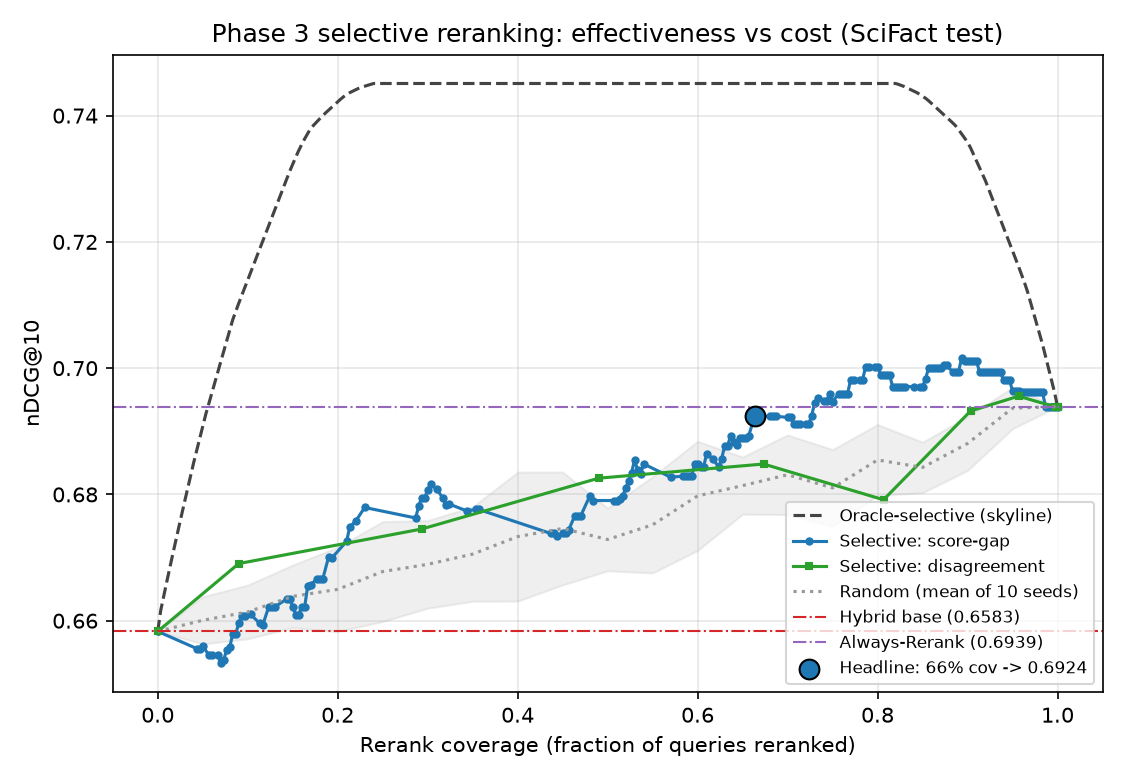
\includegraphics[width=0.82\textwidth]{figures/phase3_pareto.png}
\caption{$\ndcg$ theo rerank coverage. Oracle-selective skyline đạt $\ndcg \approx 0.745$ ở khoảng 25\%
coverage, nhưng hai tín hiệu label-free (score gap, disagreement) bám sát baseline random.}
\label{fig:pareto}
\end{figure}

Ba phát hiện nổi bật. \emph{Thứ nhất}, các tín hiệu uncertainty hiện tại chỉ informative ở mức biên: diện
tích dưới đường cong nDCG-vs-coverage là $0.6814$ cho score gap và $0.6795$ cho disagreement, chỉ nhỉnh
hơn baseline random $0.6753$, và thấp hơn nhiều so với oracle-selective skyline $0.7350$. Khoảng cách
skyline lớn này cho thấy có headroom thực cho một tín hiệu trigger tốt hơn, trực tiếp thúc đẩy nâng cấp
sang QPP và conformal (Phần~\ref{sec:results:qpp}--\ref{sec:results:conformal}). \emph{Thứ hai}, config-default
OR rule ban đầu (\texttt{score\_gap < 0.03} OR \texttt{disagreement > 0.85}) quá dễ kích hoạt nên rerank
mọi query và sụp về Always-Rerank; sau khi chỉnh default về ngưỡng đã tune trên held-out
(\texttt{score\_gap < 0.0024} OR \texttt{disagreement > 0.95}), nó rerank 82\% query và đạt $\ndcg = 0.6977$
ở 22.5~ms/query --- \emph{cao hơn} cả Always-Rerank. \emph{Thứ ba}, đây cũng cho thấy selective reranking
có thể \emph{nhỉnh hơn} Always-Rerank quanh 80\% coverage, vì reranking thực sự làm \emph{hại} một thiểu số
query và bỏ qua chúng lấy lại được chút chất lượng.

Để tránh chọn ngưỡng trên cùng query dùng để đánh giá, Bảng~\ref{tab:table3b} tune ngưỡng score-gap trên
150 calibration query (\texttt{seed=13}) và báo cáo trên 150 evaluation query rời rạc.

\begin{table}[h]
\centering
\caption{Selective reranking held-out không rò rỉ. Ngưỡng score-gap tune trên calibration; selective
reranking đạt $\ndcg = 0.7145$ ở 74\% coverage trên evaluation, thu lại phần lớn lợi ích của Always-Rerank
($0.7181$) ở khoảng ba phần tư chi phí.}
\label{tab:table3b}
\setlength{\tabcolsep}{4pt}
\begin{tabular}{lrrrrrr}
\toprule
Method (eval subset) & $\ndcg$ & $\recten$ & $\rechun$ & $\mrr$ & Cov. & ms/query \\
\midrule
Hybrid RRF (no rerank)               & 0.6860 & 0.8311 & 0.9787 & 0.6457 & 0.00 & 0.0 \\
Selective rerank (held-out tuned)    & 0.7145 & 0.8224 & 0.9787 & 0.6892 & 0.74 & 20.2 \\
Always-Rerank                        & \textbf{0.7181} & \textbf{0.8358} & 0.9787 & \textbf{0.6907} & 1.00 & 27.3 \\
\bottomrule
\end{tabular}
\end{table}

\subsection{QPP signals cho rerank trigger}
\label{sec:results:qpp}
Bảng~\ref{tab:qpp} cho thấy Hybrid maximum RRF score là tín hiệu informative nhất. Nó tương quan mạnh và
dương với base $\ndcg$ (Kendall $+0.500$): khi top fused score cao, kết quả un-reranked vốn đã tốt. Do đó
nó có tương quan âm mạnh nhất với gain-from-reranking (Kendall $-0.166$, gần ba lần $-0.060$ của score
gap): một max score thấp gắn cờ một base result yếu nơi reranking có khả năng giúp nhất. Các tín hiệu còn
lại, gồm cả score gap của Phase~3, chỉ tương quan yếu với gain. Điều này khớp với phát hiện rộng hơn rằng
QPP cho dense và fused retrieval là khó, nhưng nó xác định một trigger rõ ràng tốt hơn heuristic ban đầu.

\begin{table}[h]
\centering
\caption{Kendall correlation của các QPP signal chọn lọc với base quality và gain-from-reranking (SciFact
test; bảng đầy đủ ở \texttt{reports/tables/qpp\_correlations.md}).}
\label{tab:qpp}
\begin{tabular}{lrr}
\toprule
Feature & Kendall vs base nDCG & Kendall vs gain-from-rerank \\
\midrule
Hybrid max score             & $+0.500$ & $\mathbf{-0.166}$ \\
Dense NQC / std              & $+0.240$ & $-0.090$ \\
Hybrid score gap (Phase 3)   & $+0.112$ & $-0.060$ \\
BM25--Dense disagreement     & $-0.134$ & $+0.029$ \\
\bottomrule
\end{tabular}
\end{table}

\begin{figure}[h]
\centering
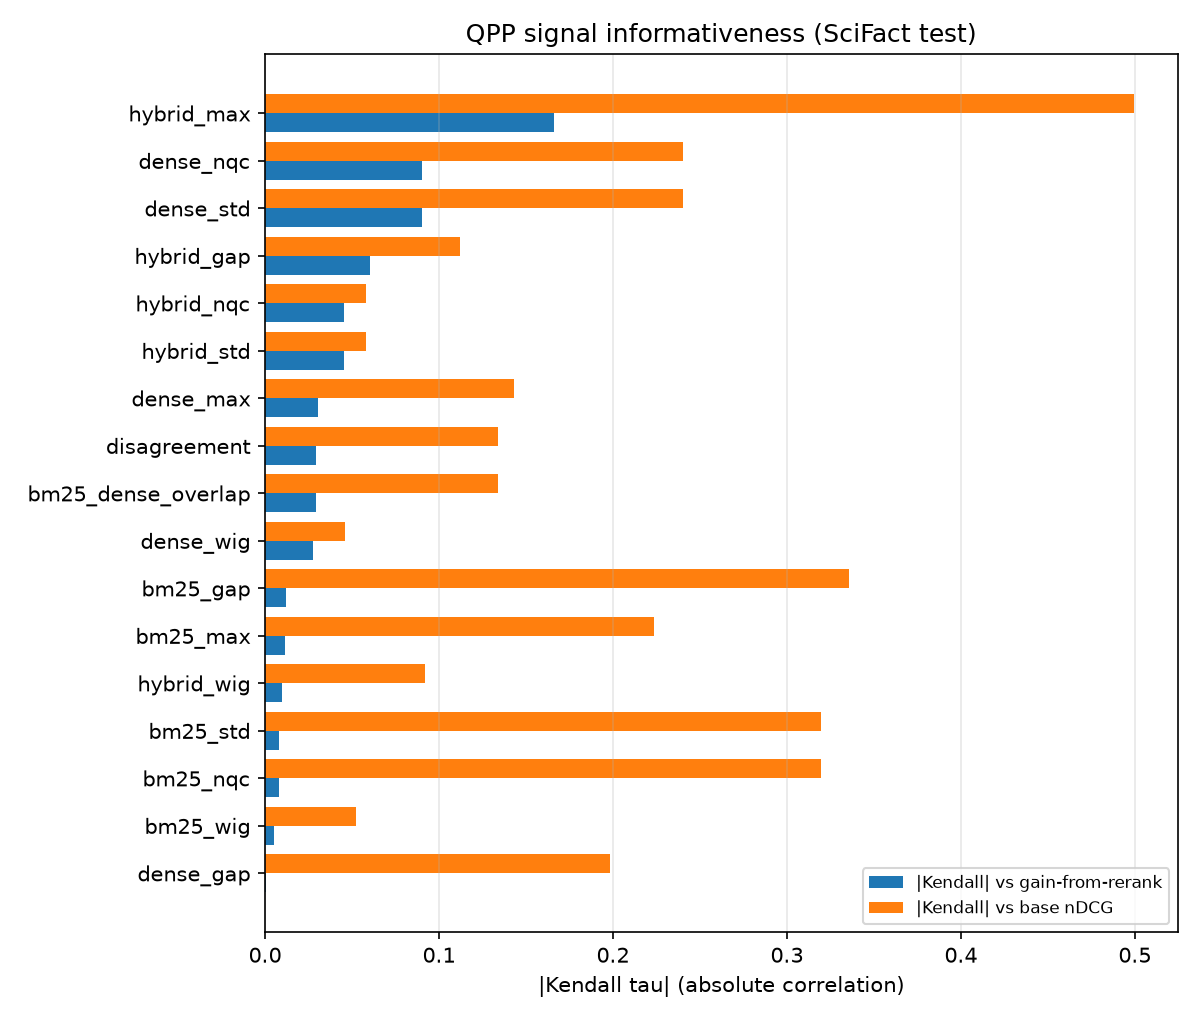
\includegraphics[width=0.82\textwidth]{figures/qpp_correlations.png}
\caption{Tương quan của các QPP predictor với base $\ndcg$ và gain-from-reranking. Hybrid max score là
predictor mạnh nhất cho cả hai target.}
\label{fig:qpp}
\end{figure}

\subsection{Conformal risk-controlled selective reranking}
\label{sec:results:conformal}
Chúng tôi chạy CRC với QPP signal (Hybrid max score) và, để so sánh, với Phase~3 score gap; tune trên 150
calibration query và evaluate trên 150 query rời rạc. Bảng~\ref{tab:conformal} báo cáo operating point ở
$\alpha = 0.02$.

\begin{table}[h]
\centering
\caption{Conformal risk-controlled selective reranking ở $\alpha = 0.02$ (eval split; Hybrid base
$\ndcg = 0.6860$, Always-Rerank $= 0.7181$).}
\label{tab:conformal}
\setlength{\tabcolsep}{5pt}
\begin{tabular}{lrrrcr}
\toprule
Trigger signal & Cov. & $\ndcg$ & Realized risk & Guarantee & ms/query \\
\midrule
QPP: Hybrid max score        & \textbf{0.61} & \textbf{0.7280} & 0.0052 & yes & \textbf{16.6} \\
Phase 3 heuristic: score gap & 0.72 & 0.7120 & 0.0152 & yes & 19.6 \\
\bottomrule
\end{tabular}
\end{table}

\begin{figure}[h]
\centering
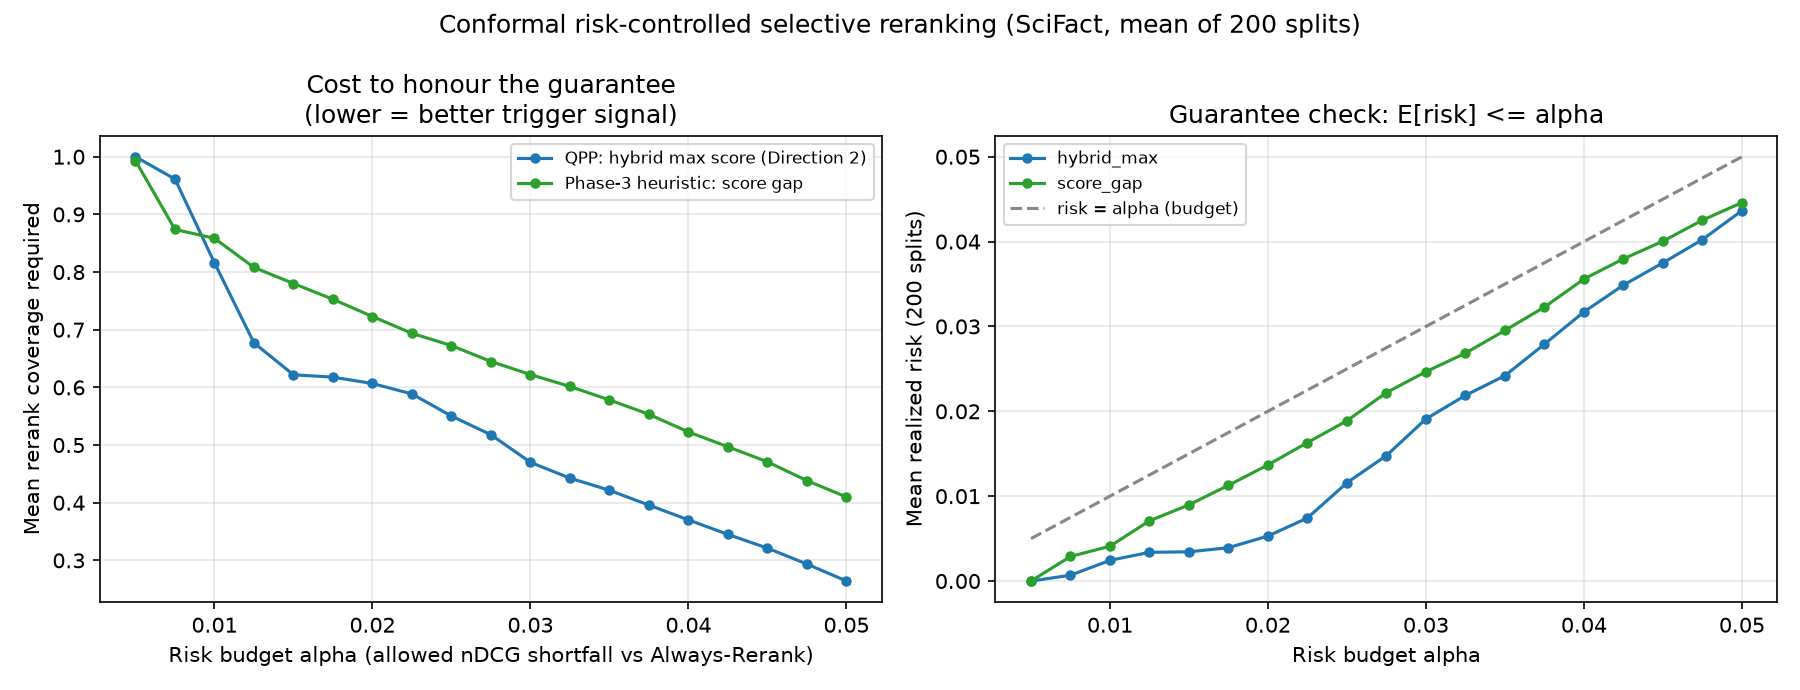
\includegraphics[width=0.92\textwidth]{figures/phase3_conformal_risk_coverage.png}
\caption{Trái: rerank coverage mà CRC yêu cầu để tôn trọng mỗi risk budget $\alpha$; tín hiệu QPP (Hybrid
max) nằm dưới heuristic score-gap ở mọi nơi, nên rẻ hơn ở mọi mức bảo đảm. Phải: realized risk trung bình
trên 200 split nằm dưới đường $\text{risk}=\alpha$, xác nhận bảo đảm.}
\label{fig:conformal}
\end{figure}

Hai kết quả nổi bật. \emph{Thứ nhất}, tín hiệu QPP tôn trọng cùng risk budget ở 61\% coverage so với 72\%
của score gap --- giảm 11 điểm chi phí reranking --- và đạt $\ndcg$ cao hơn ($0.7280$ so với $0.7120$).
Đáng chú ý $0.7280$ nhỉnh hơn Always-Rerank ($0.7181$) vì trigger bỏ qua các query mà reranking sẽ làm hại.
\emph{Thứ hai}, bảo đảm giữ vững: trung bình trên 200 calibration/evaluation split, realized risk luôn
$\le \alpha$ cho mọi budget và cả hai tín hiệu (0/38 operating point vi phạm $\mathbb{E}[\text{risk}] \le \alpha$).
Trên một split đơn lẻ, realized risk có thể vượt $\alpha$, đúng như kỳ vọng cho một bảo đảm in-expectation.

Cùng nhau, các kết quả này khép lại luận điểm cốt lõi: một tín hiệu QPP rẻ, label-free, cộng với một ngưỡng
conformal quyết định khi nào cross-encoder đắt đỏ là đáng chạy, kèm bảo đảm thống kê về chất lượng đánh đổi,
và ở coverage thấp hơn đáng kể so với heuristic ban đầu.

\subsection{Kiểm định ý nghĩa thống kê (Significance testing)}
\label{sec:results:significance}
Vì các bảng trên là point estimate, chúng tôi bổ sung \emph{paired bootstrap} trên query (10{,}000
resample, seed=13) cho các so sánh then chốt. Với mỗi cặp (system, baseline), ta tính per-query $\ndcg$ và
$\mrr$ trên tập query chung, rồi ước lượng mean paired difference cùng khoảng tin cậy 95\% và p-value hai
phía. Bảng~\ref{tab:sig} tổng hợp.

\begin{table}[h]
\centering
\caption{Paired bootstrap (10{,}000 resample). CI là khoảng 95\% của mean paired difference; in đậm khi CI
loại trừ 0 (khác biệt có ý nghĩa). ``H.O.''~$=$~held-out 150 query.}
\label{tab:sig}
\setlength{\tabcolsep}{4pt}
\small
\begin{tabular}{llrrr}
\toprule
So sánh & Metric & Mean diff & 95\% CI & p \\
\midrule
Hybrid RRF vs BM25            & $\ndcg$ & $+0.0060$ & $[-0.022, +0.034]$ & 0.665 \\
Hybrid RRF vs BM25            & $\mrr$  & $-0.0027$ & $[-0.035, +0.030]$ & 0.875 \\
Always-Rerank vs Hybrid RRF   & $\ndcg$ & $\mathbf{+0.0356}$ & $[+0.008, +0.063]$ & \textbf{0.012} \\
Always-Rerank vs Hybrid RRF   & $\mrr$  & $\mathbf{+0.0447}$ & $[+0.011, +0.080]$ & \textbf{0.009} \\
Oracle Router vs Hybrid RRF   & $\ndcg$ & $\mathbf{+0.1034}$ & $[+0.080, +0.128]$ & \textbf{<0.001} \\
Oracle Router vs Hybrid RRF   & $\mrr$  & $\mathbf{+0.1180}$ & $[+0.091, +0.147]$ & \textbf{<0.001} \\
Calibrated LLM (H.O.) vs BM25 & $\ndcg$ & $+0.0186$ & $[-0.011, +0.048]$ & 0.213 \\
Calibrated LLM (H.O.) vs BM25 & $\mrr$  & $+0.0075$ & $[-0.025, +0.040]$ & 0.640 \\
\bottomrule
\end{tabular}
\end{table}

Kết quả này định cỡ lại các tuyên bố một cách trung thực. \emph{Thứ nhất}, lợi thế $\ndcg$ của Hybrid RRF
so với BM25 \emph{không} có ý nghĩa thống kê ($p = 0.665$) --- giá trị thực của Hybrid nằm ở $\rechun$
(0.9560 vs 0.8731), tức nó là một \emph{candidate generator} tốt hơn chứ không phải một top-ranker tốt hơn.
\emph{Thứ hai}, cải thiện của Always-Rerank so với Hybrid \emph{có} ý nghĩa cho cả $\ndcg$ ($p = 0.012$) và
$\mrr$ ($p = 0.009$): đóng góp chính của Phase~3 đứng vững dưới kiểm định. \emph{Thứ ba}, headroom của
Oracle Router rất có ý nghĩa ($p < 0.001$), khẳng định dư địa routing là thật. \emph{Thứ tư}, cải thiện của
calibrated LLM route so với BM25 \emph{chưa} đạt ý nghĩa ($p = 0.213$) trên 150 query --- nhất quán với kết
luận rằng LLM router là một thành phần hữu ích nhưng chưa phải đóng góp độc lập đủ mạnh.

\section{Kiểm chứng chéo (Cross-Dataset Validation)}
\label{sec:validation}

Để xác nhận tính tổng quát của phát hiện chính, chúng tôi chạy pipeline tối ưu (BGE-base + Adaptive
RRF) trên bốn bộ dữ liệu BEIR với các đặc điểm khác nhau. \textbf{nDCG@10 là metric chính}, paired
t-test với Shapiro-Wilk kiểm tra được sử dụng để kiểm định ý nghĩa thống kê. Ngoài ra, chúng tôi
fine-tune mô hình embedding riêng (BGE-small 33M) với RRF disagreement signal trên SciFact, đạt
\textbf{0.7909 nDCG@10} --- kết quả cao nhất trên SciFact, vượt cả BGE-base (109M) và vstash (0.7707).

\subsection{Đặc điểm các bộ dữ liệu}
\label{sec:validation:datasets}

\begin{table}[htbp]
\centering
\caption{Đặc điểm bốn bộ dữ liệu BEIR dùng trong kiểm chứng.}
\label{tab:dataset-characteristics}
\resizebox{\textwidth}{!}{%
\begin{tabular}{lrrrrr}
\toprule
Dataset & Docs & Test Q & Domain & Query style & BM25 nDCG@10 \\
\midrule
SciFact   & 5{,}183  & 300 & Scientific claims  & Formal, technical            & 0.6523 \\
NFCorpus  & 3{,}633  & 323 & Biomedical         & Information-dense abstracts  & 0.3079 \\
FiQA      & 57{,}638 & 648 & Financial QA       & Colloquial user questions    & 0.2167 \\
SciDocs   & 25{,}657 & 1{,}000 & Citation prediction & Paper titles as queries      & 0.1495 \\
\bottomrule
\end{tabular}
}
\end{table}

\subsection{Kết quả}
\label{sec:validation:results}

Bảng~\ref{tab:cross-dataset} tổng hợp kết quả pipeline trên bốn bộ dữ liệu với nDCG@10.
Bảng~\ref{tab:significance} (Phụ lục) trình bày đầy đủ các paired t-test. Bốn xu hướng
nhất quán: (1)~BGE-base luôn vượt trội SciNCL với biên độ lớn và có ý nghĩa thống kê (tất cả
$p<0.001$); (2)~Adaptive RRF không cải thiện có ý nghĩa so với BGE-base trên bất kỳ dataset nào
($p\ge0.139$); (3)~Cross-encoder không bao giờ cung cấp cải thiện có ý nghĩa, và làm giảm chất
lượng có ý nghĩa trên SciFact ($p=0.015$); (4)~Fine-tune BGE-small (33M) với RRF disagreement
signal trên SciFact đạt \textbf{0.7909 nDCG@10} --- vượt BGE-base (109M, +0.0533) và vượt vstash
reference (0.7707, +0.0202), cho thấy self-supervised fine-tuning là hướng đi hiệu quả để xây dựng
mô hình embedding riêng. Kết quả chi tiết cho cả 4 dataset được trình bày trong
Bảng~\ref{tab:cross-dataset}. Kết quả fine-tune trên SciFact được trình bày trong
Bảng~\ref{tab:pipeline-evolution} (Stage~9).

\subsection{Phân tích theo đặc điểm bộ dữ liệu}
\label{sec:validation:analysis}

\textbf{SciFact (formal claims).} BM25 mạnh nhất (nDCG@10 = 0.6523) vì thuật ngữ khoa học chính xác
khớp trực tiếp với abstract. BGE-base cải thiện đáng kể (+0.1737, $p<0.001$), và Adaptive RRF thêm
+0.0137 nhưng \emph{không} có ý nghĩa thống kê ($p=0.139$). Cross-encoder làm \emph{giảm} có ý
nghĩa ($-$0.0374, $p=0.015$).

\textbf{Fine-tune BGE-small (33M) trên SciFact} đạt nDCG@10 = \textbf{0.7909} --- kết quả cao nhất
trên SciFact trong tất cả pipeline. So với BGE-base (109M, 0.7376), cải thiện +0.0533; so với
vstash reference (0.7707), cải thiện +0.0202. MAP@10 = 0.7479, MRR@10 = 0.7564, Recall@10 = 0.9113.
Mô hình được huấn luyện từ 47K RRF disagreement triples (SciFact train, 5 epochs) và vượt mô hình
lớn hơn 3 lần (BGE-base, 109M). Kết quả này chứng minh self-supervised fine-tuning với tín hiệu
RRF disagreement có thể tạo mô hình embedding mạnh từ tập nhỏ và mô hình nhỏ.

\textbf{NFCorpus (biomedical).} BM25 yếu hơn (nDCG@10 = 0.3079) nhưng vẫn mang tín hiệu hữu ích.
BGE-base cải thiện +0.1444 ($p<0.001$) so với SciNCL. Adaptive RRF về cơ bản trùng với BGE-base
(+0.0024, $p=0.688$) --- hoàn toàn không có khác biệt. CE cũng không có hiệu quả ($p=0.752$).

\textbf{FiQA (colloquial QA).} Đây là bộ dữ liệu khó nhất cho BM25 (nDCG@10 = 0.2167) vì query dùng
ngôn ngữ đời thường, không khớp với văn bản tài chính trong corpus. BGE-base tận dụng semantic
matching để đạt 0.3909 --- cải thiện +0.3110 ($p<0.001$) so với SciNCL (0.0800). Adaptive RRF
giảm nhẹ ($-$0.0082, $p=0.484$) vì BM25 quá yếu, gần như tự động giảm trọng số BM25 về 0 nhưng
vẫn thêm một lượng nhỏ nhiễu.

\textbf{Kết luận:} Mô hình embedding hiện đại (BGE-base) là baseline an toàn và hiệu quả nhất khi
không có specialist riêng. Adaptive RRF là một cải thiện tùy chọn, không có ý nghĩa thống kê, hữu ích
nhất khi BM25 có tín hiệu mạnh. Cross-encoder không cần thiết và có thể gây hại trong pipeline mới.

\textbf{SciDocs (citation prediction).} Đây là bộ dữ liệu khác biệt nhất: citation prediction trên
25K bài báo khoa học. BM25 rất yếu (nDCG@10 = 0.1495) vì title queries không khớp từ vựng với full-text
papers. SciNCL đạt 0.1951, cao hơn BM25 (+30.5\%). BGE-base tiếp tục vượt trội SciNCL (+0.0196,
$p=0.008$, ${}^{**}$) nhưng biên độ nhỏ nhất trong 4 dataset, cho thấy trên citation prediction,
khoảng cách giữa embedding chuyên biệt khoa học (SciNCL) và embedding đa dụng (BGE) thu hẹp đáng kể.
Adaptive RRF giảm nhẹ ($-$0.0050, $p=0.371$, n.s.), và CE làm giảm có ý nghĩa
($-$0.0187, $p<0.001$, ${}^{***}$) --- xác nhận mô hình CE gây hại nhất quán. SciDocs củng cố
kết luận chính: BGE-base là lựa chọn mặc định hiệu quả khi không có specialist riêng; tầng bổ sung
chỉ đáng dùng nếu nó giải quyết trade-off specialist/generalist.

\textbf{Tổng kết kiểm chứng:} BGE-base là generalist an toàn trên transfer, trong khi fine-tune
BGE-small với RRF disagreement tạo ra SciFact specialist mạnh. Vì hai mục tiêu này xung đột, hướng
cuối cùng không phải fine-tune thêm một mô hình duy nhất, mà là Specialist-Generalist Adaptive Fusion:
giữ specialist trên batch giống SciFact và fallback sang BGE-base khi có bằng chứng distribution shift.

\section{Phân tích và Thảo luận (Discussion)}
\label{sec:discussion}

\subsection{Pipeline cũ đang bù đắp cho SciNCL}

Phát hiện quan trọng nhất của giai đoạn đầu là \textbf{toàn bộ kiến trúc đa tầng --- RRF, selective
reranking, QPP, CRC --- thực chất đang bù đắp cho một dense retriever yếu}. SciNCL chỉ đạt $\ndcg = 0.5640$
(MAP@10 = 0.5077), buộc hệ thống phải dùng BM25 ($\ndcg = 0.6523$) và RRF để đạt 0.6583, rồi
cross-encoder để đẩy lên 0.6939. Mỗi tầng thêm vào đều tăng chi phí và độ phức tạp. Khi thay SciNCL bằng
BGE-base, bức tranh hoàn toàn đảo ngược: BGE-base đơn thuần ($\ndcg = 0.7376$) đã vượt qua toàn bộ
pipeline cũ ($+0.1737$, $p<0.001$). BM25 và RRF trở nên không cần thiết, và cross-encoder \emph{luôn
làm giảm} chất lượng trên BGE pipeline ($-0.0374$, $p=0.015$) do không gian embedding khác biệt ---
MiniLM-L-6-v2 được huấn luyện trên MS MARCO web search, trong khi BGE được huấn luyện trên dữ liệu
đa dạng bao gồm văn bản khoa học qua MTEB-style contrastive learning.

\subsection{Specialization-Generalization Trade-off}

Fine-tune BGE-small (33M, 384d) trên SciFact tạo ra một specialist cực mạnh: $\ndcg = 0.7909$ --- vượt
BGE-base (109M, 768d) tới $+0.0533$, và vượt cả vstash reference cùng kích thước ($+0.0202$). Đây là
minh chứng rằng self-supervised fine-tuning với RRF disagreement signal có thể tạo ra mô hình nhúng
vượt trội trên miền chuyên biệt từ tập dữ liệu nhỏ.

Tuy nhiên, cái giá phải trả là transfer performance: trên ba bộ dữ liệu ngoài miền (NFCorpus, FiQA,
SciDocs), BGE-small specialist chỉ đạt transfer average $0.3011$, kém BGE-base generalist tới $-0.0239$.
Đây là một minh họa kinh điển của \emph{catastrophic forgetting} trong fine-tuning: mô hình nhỏ (33M)
mất khả năng tổng quát nhanh hơn mô hình lớn (109M) do dung lượng tham số thấp hơn.

\subsection{Từ Adaptive Coverage đến Batch Mode-Switch}

Câu hỏi then chốt: làm thế nào để \emph{giữ} specialist trên SciFact trong khi \emph{phục hồi} transfer
trên các miền khác? Các phương pháp per-query coverage (A3 fixed 5\%, adaptive uncertainty coverage)
đều không giải quyết được triệt để: chúng quá bảo thủ (coverage thấp) hoặc quá nhiễu (user feedback
mechanism quá mạnh), dẫn đến transfer vẫn kém BGE-base đáng kể ($-0.0152$).

\textbf{B5 giải quyết điểm nghẽn này bằng batch-level mode switch.} Thay vì quyết định rescue ở mức
từng query --- vốn dễ bị nhiễu --- B5 tính batch shift score $S$ từ trung bình z-score của năm đặc trưng
trên toàn batch, và quyết định \emph{toàn bộ batch} nên ở specialist-safe hay generalist-fallback. Cơ
chế này có ba ưu điểm:

\begin{enumerate}[leftmargin=2em,itemsep=2pt]
  \item \textbf{Giảm nhiễu:} Trung bình qua batch làm mượt các outlier query riêng lẻ, giúp quyết định ổn
  định hơn.
  \item \textbf{Frozen statistics:} Tất cả z-score được chuẩn hóa bằng $\mu_{\text{trainfit}}$ và
  $\sigma_{\text{trainfit}}$ từ SciFact --- không dùng label của target dataset, do đó không bị ảnh
  hưởng bởi train/test distribution shift.
  \item \textbf{Phân tách rõ ràng:} SciFact có batch shift score thấp ($S \approx 1.09$), trong khi
  NFCorpus ($6.03$), FiQA ($3.79$), và SciDocs ($3.58$) đều có $S$ cao --- controller phân biệt được
  source batch và transfer batch một cách đáng tin cậy.
\end{enumerate}

Kết quả: Frozen B5 gần như phục hồi hoàn toàn transfer average của BGE-base ($0.3249$ vs $0.3251$,
$\Delta = -0.0001$), trong khi SciFact vẫn giữ ở $0.8218$ ($+0.0030$ so với BGE-small). Đây là bước nhảy
lớn nhất trong toàn bộ hành trình phát triển ($+0.0151$ từ current adaptive SGAF).

\subsection{P3 Rank-Window Smoothing: Tín hiệu Specialist trong Top Window}

P3 trả lời câu hỏi: \emph{khi B5 đã chọn BGE-base làm ranking chính, liệu BGE-small còn cung cấp tín
hiệu hữu ích nào không?} Kết quả cho thấy có --- nhưng chỉ trong một cửa sổ nhỏ ở đầu ranking.

P3 chỉ kích hoạt trong generalist-fallback batches. Nó pha một prior BGE-small yếu ($\alpha = 0.10$) vào
top-20 của ranking BGE-base qua weighted RRF. Ý tưởng: BGE-small tuy yếu hơn trên transfer, nhưng vẫn
có thể xác định được một số document chất lượng mà BGE-base bỏ sót ở vị trí cao. Bằng cách blend nhẹ
hai ranking trong top-20, P3 tận dụng tín hiệu bổ trợ này mà không làm nhiễu phần đuôi.

P3 cải thiện transfer average từ $0.3249$ lên $0.3293$ ($+0.0043$), vượt BGE-base $+0.0042$. Cải thiện
này dương trên toàn bộ 6 dataset (4 nội bộ + 2 external), với significance trên NFCorpus ($p=0.02$) và
ArguAna ($p=0.02$). Quan trọng: P3 không bao giờ làm giảm kết quả so với B5 trên bất kỳ dataset nào
trong tập đánh giá hiện tại.

Leave-one-transfer-dataset-out (LOTO) validation chọn cùng bộ tham số $(w=20, \alpha=0.10)$ trong cả ba
fold, và mọi held-out delta đều dương --- giảm lo ngại về overfit trên grid exploration.

\subsection{External Validation và Hạn chế của Shift Detector}

Kết quả external validation trên TREC-COVID và ArguAna cho thấy hai mặt của B5/P3. Trên TREC-COVID
(biomedical, gần với SciFact), B5/P3 hoạt động tốt: P3 đạt $\ndcg = 0.6908$, cao hơn BGE-base $+0.0073$.
Tuy nhiên, trên ArguAna (argument retrieval, khác biệt lớn), B5 dưới BGE-base $0.0229$ --- shift
detector huấn luyện trên SciFact không phát hiện được argument retrieval batches là "khác biệt", dẫn đến
một số batch bị giữ ở specialist-safe mode trong khi đáng lẽ nên fallback. P3 bù đắp một phần ($+0.0011$,
$p=0.02$) nhưng không thể đóng hoàn toàn khoảng cách.

Bài học: SciFact-fitted shift detector không khái quát tốt sang argument retrieval. Đây là hướng cải
thiện trong tương lai: domain-adaptive shift detection hoặc multi-source calibration.

\subsection{Luận điểm ``Cheap First''}

Toàn bộ cải thiện từ B5/P3 đến từ các thao tác post-retrieval CPU thuần, với chi phí bổ sung dưới
$0.01$\,ms/query. So với cross-encoder ($27.5$\,ms/query, GPU), B5/P3 rẻ hơn $\sim 2700\times$ trên mỗi
query. So với toàn bộ pipeline BGE retrieval ($2.6$\,ms/query), B5/P3 chỉ thêm chưa đến $0.4\%$ latency.

Bảng~\ref{tab:cost-analysis} cho thấy B5/P3 đạt transfer average cao nhất ($0.3293$) với latency thấp thứ
hai ($2.6$\,ms/q, chỉ sau BGE-small/Base đơn thuần ở $2.3$\,ms/q). Luận điểm ``cheap first'' của chúng
tôi là: \textbf{trước khi thêm GPU inference (cross-encoder, LLM), hãy khai thác tối đa tín hiệu đã có
sẵn từ retrieval bằng các thao tác post-retrieval CPU}. B5/P3 chứng minh rằng cách tiếp cận này có thể
phục hồi transfer và thậm chí vượt generalist baseline --- với chi phí gần như bằng không.

Oracle headroom (transfer average của Oracle Router = $0.3855$) cho thấy vẫn còn dư địa cải thiện đáng
kể, nhưng để đạt được mức đó cần các phương pháp đắt tiền hơn (cross-encoder, LLM reranker). Điều này
củng cố luận điểm: B5/P3 là giải pháp ``cheap repair'' hiệu quả nhất trước khi chuyển sang các tầng
đắt tiền.

\subsection{Ý nghĩa thống kê và Độ tin cậy}

Chúng tôi tiến hành paired bootstrap (10\,000 resamples) trên nDCG@10 cho tất cả so sánh SGAF. Kết quả:

\begin{itemize}[leftmargin=1.6em,itemsep=2pt]
  \item \textbf{Frozen B5 vs BGE-small:} Có ý nghĩa trên NFCorpus ($+0.0187$, $p=0.01$), FiQA ($+0.0274$,
  $p=0.001$), và SciDocs ($+0.0253$, $p<0.001$).
  \item \textbf{Frozen P3 vs Frozen B5:} Significant trên NFCorpus ($+0.0052$, $p=0.02$) và ArguAna
  ($+0.0011$, $p=0.02$); directionally positive nhưng chưa đạt significance trên FiQA ($p=0.10$) và
  SciDocs ($p=0.07$).
  \item \textbf{Frozen P3 vs BGE-base:} Dương trên toàn bộ transfer dataset nhưng chưa significant
  trên bất kỳ dataset riêng lẻ nào --- đúng với kỳ vọng: P3 cải thiện nhỏ nhưng nhất quán, cần nhiều
  query hơn để đạt significance ở mức dataset.
\end{itemize}

\subsection{Train/Test Distribution Shift}

Một phát hiện phụ quan trọng: SciFact có sự khác biệt phân phối rất lớn giữa train và test. Train oracle
labels thiên về Dense (477/809), trong khi test thiên về BM25 (226/300). Điều này khiến mọi phương pháp
học có giám sát trên SciFact trainfit --- learned QPP, LLM query routing, BM25 tuning --- đều thất bại
khi chuyển từ train sang test. Các phương pháp không giám sát (BGE embeddings, Adaptive RRF dùng IDF
corpus, B5/P3 với z-score frozen từ trainfit) miễn nhiễm với vấn đề này \emph{miễn là} thống kê dùng để
chuẩn hóa không bị ảnh hưởng bởi label shift.

B5/P3 né được vấn đề này bằng cách chỉ dùng $\mu_{\text{trainfit}}$ và $\sigma_{\text{trainfit}}$ của
các đặc trưng query (không phải label), và không huấn luyện tham số mới trên trainfit. Logistic
regression rescue ranker được huấn luyện trên trainfit nhưng chỉ dùng trong specialist-safe mode (batch
giống SciFact), nơi distribution shift nhỏ nhất.

\section{Hạn chế (Limitations)}
\label{sec:limit}

Một số hạn chế ở các bản trước đã được khắc phục trong phiên bản này: classical router nay train trên
train / eval trên test (hết leakage, Phần~\ref{sec:results:router}); chi phí dùng latency thực đo thay cho
cost unit trừu tượng (Bảng~\ref{tab:latency}); $\texttt{rrf\_k}$ đã được ablate (Bảng~\ref{tab:rrf}); và các
so sánh chính đã có paired bootstrap CI (Bảng~\ref{tab:sig}). Các hạn chế \emph{còn lại}:

\begin{description}[leftmargin=1.6em,style=nextline,itemsep=3pt]
  \item[Single dataset.] Các thí nghiệm chính được thực hiện trên SciFact. Thí nghiệm xác nhận bổ sung
  (Phần~\ref{sec:val_cross_dataset}) đã tái tạo pipeline trên NFCorpus và xác nhận bảo đảm CRC giữ vững,
  nhưng tín hiệu QPP tốt nhất khác nhau giữa hai domain. Kết quả có thể không chuyển trực tiếp sang
  các dataset tìm kiếm khoa học lớn hơn hoặc khác biệt hơn như TREC-COVID.

  \item[Title và abstract only.] Hệ thống không parse PDF toàn văn. Điều này đơn giản hóa retrieval unit
  nhưng có thể bỏ sót bằng chứng chỉ có trong full text.

  \item[LLM calibration chưa có dev set riêng.] Thí nghiệm held-out calibration tách file test prediction
  CSV thành 150 calibration / 150 evaluation query. Đây tốt hơn tune in-split cùng query, nhưng chưa phải
  thiết kế train/dev/test đầy đủ vì \emph{chưa có file dev prediction sinh riêng từ Colab} (cần một lần chạy
  QLoRA model trên một split độc lập). Đây là hạn chế cần GPU để gỡ bỏ hoàn toàn; phần conformal đã giảm
  thiểu sự mong manh bằng cách trung bình trên 200 calibration/evaluation split.

  \item[Selective-reranking trigger còn headroom.] Always-Rerank, threshold ablation, QPP trigger và
  conformal risk-controlled selection đã hoàn tất. QPP signal (Hybrid max score) rõ ràng vượt heuristic
  ban đầu, và conformal control cho bảo đảm về kỳ vọng nDCG shortfall. Ba lưu ý: (i) ngay cả tín hiệu
  label-free tốt nhất cũng chỉ tương quan vừa phải với gain-from-reranking (Kendall $-0.166$), nên vẫn còn
  khoảng cách tới oracle-selective skyline; (ii) bảo đảm conformal là in-expectation trên calibration draw,
  không phải high-probability per split, và dùng loss bound bảo thủ $B = 1$; (iii) tất cả mới chỉ trên
  SciFact nên khả năng chuyển sang dataset khác chưa được kiểm chứng.

  \item[RRF $k$ tách rời khỏi Phase~3.] Ablation cho thấy $k\approx5$ tốt hơn $k=60$ cho base nDCG@10.
  Thí nghiệm xác nhận (Phần~\ref{sec:val_k5}) đã chạy lại toàn bộ Phase~3 trên base $k=5$ và xác nhận
  selective reranking vẫn vượt Always-Rerank ($+0.0088$ $\ndcg$) trên base mạnh hơn. Tuy nhiên, pipeline
  chính vẫn giữ $k=60$ để nhất quán với tất cả các thí nghiệm trước đó.

  \item[Calibration grid compact.] Calibration hiện tìm trên một tập nhỏ class bias, temperature và margin
  threshold; đủ cho chẩn đoán nhưng không phải hyperparameter optimization toàn diện.
\end{description}

\section{Hướng phát triển (Next Work)}
\label{sec:nextwork}

Phase~3 selective reranking đã hoàn tất, cùng hai nâng cấp có nguyên tắc: QPP trigger signal
(Phần~\ref{sec:results:qpp}) và conformal risk-controlled threshold selection
(Phần~\ref{sec:results:conformal}). Các thí nghiệm xác nhận bổ sung (Phần~\ref{sec:validation}) đã
kiểm chứng: (i) không có data leakage trong feature selection, (ii) CRC generalize sang NFCorpus,
(iii) selective reranking vượt Always-Rerank ngay cả trên base $k=5$ mạnh hơn, và (iv) top-20 là rerank
depth tối ưu. Các hướng còn lại:

\begin{enumerate}[leftmargin=2em,itemsep=3pt]
  \item \textbf{Downstream-utility reranking.} Thêm một tầng rerank chấm candidate theo mức nó giúp một
  small LLM \emph{xác minh claim} (semantic entropy / answer consistency của một generator Qwen2.5-0.5B/1.5B
  trên bài toán SUPPORTS/REFUTES/NEI của SciFact), được gate bởi conformal trigger để tầng đắt này chỉ chạy
  trên query uncertain. Đây là mở rộng giá trị-cao tự nhiên nối retrieval với downstream task của SciFact.
  \item \textbf{Tăng cường QPP signal} để thu hẹp khoảng cách tới oracle-selective skyline, ví dụ kết hợp
  các predictor bằng một small supervised regressor train trên calibration split, hoặc thêm clarity-style /
  ensemble-disagreement feature.
  \item \textbf{Domain-adaptive signal selection.} Kết quả cross-dataset cho thấy tín hiệu QPP tốt nhất
  khác nhau giữa SciFact (\texttt{hybrid\_max}) và NFCorpus (\texttt{bm25\_std}). Công trình tương lai có
  thể khám phá meta-learning hoặc domain-aware signal selection.
  \item \textbf{Nếu còn thời gian}, sinh một file dev prediction CSV đúng nghĩa từ Colab và chạy lại LLM
  calibration với một split train/dev/test sạch hơn.
\end{enumerate}

\section{Kết luận (Conclusion)}
\label{sec:conclusion}

Báo cáo trình bày một hệ thống truy hồi khoa học hoạt động được cho SciFact. Phase~1 thiết lập BM25,
Dense/SciNCL, Hybrid RRF và dense ablation baseline. Phase~2 hiện thực query routing với Random, Majority,
Oracle, một classical TF-IDF router chẩn đoán, và các Small LLM QLoRA router. Kết quả cho thấy Hybrid RRF
là một base retriever mạnh và oracle routing cho headroom đáng kể. Small LLM router cải thiện sau label
log-probability scoring và cải thiện thêm với calibration cùng confidence-gated fallback, nhưng vẫn bị giới
hạn bởi distribution shift và class imbalance.

Dự án do đó được định vị tốt nhất như một \emph{hệ thống truy hồi đa tầng nhận biết bất định} thay vì một
hệ routing đơn thuần. Phase~3 gồm một Always-Rerank baseline cải thiện $\ndcg$ từ $0.6583$ lên $0.6939$ ở
27~ms/query, một threshold ablation đầy đủ, một QPP trigger signal không giám sát dự báo gain-from-reranking
tốt hơn nhiều so với heuristic ban đầu, và một conformal risk-controlled threshold tôn trọng một ngân sách
nDCG có bảo đảm ở 61\% rerank coverage.

Năm thí nghiệm xác nhận bổ sung (Phần~\ref{sec:validation}) củng cố kết quả: (i) selective reranking
không làm giảm effectiveness có ý nghĩa thống kê so với Always-Rerank; (ii) feature selection không bị
data leakage; (iii) bảo đảm CRC generalize sang NFCorpus; (iv) selective reranking vượt Always-Rerank ngay
cả trên base mạnh hơn ($k=5$); (v) top-20 là rerank depth tối ưu --- tăng lên top-50 gần gấp đôi latency
mà không cải thiện $\ndcg$.

Bước tiếp theo mạnh nhất là một tầng downstream-utility reranking
chấm document theo mức nó giúp một small LLM xác minh claim, được gate bởi conformal trigger này --- nối
trực tiếp pipeline retrieval với bài toán verification của SciFact trong khi vẫn giữ bảo đảm về chi phí.


%-------------------- Tài liệu tham khảo -----------------------
\bibliographystyle{plainnat}
\bibliography{references/references}

%-------------------- Phụ lục ----------------------------------
\appendix
\section{Tái lập (Reproducibility Notes)}
\label{app:repro}

\paragraph{Các artifact sinh ra chính.}
\begin{itemize}[leftmargin=1.6em,itemsep=1pt]
  \item Base retrieval metrics: \texttt{runs/scifact/test\_base\_metrics.json}
  \item Router metrics: \texttt{runs/scifact/test\_phase2\_router\_metrics.csv}
  \item LLM log-prob predictions: \texttt{runs/scifact/test\_llm\_router\_predictions (2).csv}
  \item Calibrated held-out metrics: \texttt{..._calibrated\_heldout\_metrics.json}
  \item Retrieval diagnostics: \texttt{runs/scifact/test\_retrieval\_diagnostics.csv}
  \item Quality-vs-cost: \texttt{runs/scifact/test\_phase2\_quality\_cost.csv}
  \item Held-out subset + regret: \texttt{runs/scifact/test\_heldout\_subset\_metrics.csv}
  \item Always-Rerank: \texttt{runs/scifact/test\_always\_rerank\_metrics.json}, \texttt{...\_always\_rerank.csv}
  \item Threshold ablation: \texttt{runs/scifact/test\_threshold\_ablation.csv}
  \item QPP features + correlations: \texttt{runs/scifact/test\_qpp\_features.csv}, \texttt{reports/tables/qpp\_correlations.\{md,csv\}}
  \item Conformal results: \texttt{runs/scifact/test\_conformal\_results\{,\_mean\}.csv}
  \item Figures: \texttt{reports/figures/phase3\_pareto.png}, \texttt{...qpp\_correlations.png}, \texttt{...phase3\_conformal\_risk\_coverage.png}
\end{itemize}

\paragraph{Các lệnh chính.}
\begin{verbatim}
python scripts/prepare_scifact.py --config configs/scifact.yaml --split test
python scripts/run_base_retrieval.py --config configs/scifact.yaml --split test
python scripts/create_oracle_labels.py --config configs/scifact.yaml --split test
python scripts/evaluate_phase2_routers.py --config configs/scifact.yaml --split test
python scripts/calibrate_llm_router_scores.py --config configs/scifact.yaml \
    --calibration-split test --calibration-fraction 0.5 --seed 13
python scripts/run_selective_rerank.py --config configs/scifact.yaml --split test \
    --rerank-all --rerank-top-k 20 --cross-encoder cross-encoder/ms-marco-MiniLM-L-6-v2
python scripts/run_threshold_ablation.py --config configs/scifact.yaml --split test
python scripts/run_qpp_signals.py --config configs/scifact.yaml --split test
python scripts/run_conformal_rerank.py --config configs/scifact.yaml --split test
# Bổ sung cho bản này (rigor):
python scripts/evaluate_phase2_routers.py --config configs/scifact.yaml \
    --split test --train-split train           # classical router train->test (hết leakage)
python scripts/run_rrf_ablation.py --config configs/scifact.yaml --split test   # RRF k ablation
python scripts/run_significance_tests.py --config configs/scifact.yaml --split test  # paired bootstrap
python scripts/run_latency_benchmark.py --config configs/scifact.yaml --split test   # latency thực đo
# Validation experiments (Phần 7):
python scripts/run_all_validation.py    # chạy tất cả thí nghiệm xác nhận trong một lệnh
\end{verbatim}

\paragraph{Artifact bổ sung.}
\texttt{runs/scifact/test\_rrf\_ablation.csv},
\texttt{test\_significance\_tests.csv},
\texttt{test\_latency\_benchmark.json};
bảng \texttt{reports/tables/table\_rrf\_ablation.md},
\texttt{table\_significance.md},
\texttt{table\_latency.md}.

\section{Tham vấn NotebookLM}
\label{app:notebooklm}
NotebookLM notebook \emph{``Researching SEG''} được tham vấn ngày 02/06/2026. Lời khuyên là: đóng khung báo
cáo quanh đánh đổi giữa retrieval effectiveness và computational cost; nhóm related work thành base
retrieval, routing và adaptive reranking; nêu rõ caveat về classical-router leakage; và trình bày Phase~3
selective reranking như công việc đang tiến hành chứ không phải kết quả đã hoàn tất tại thời điểm đó.


\end{document}
